% Seminarul 1: Date, randamente și indicatori
% Statistica piețelor financiare -- Program de licență, Academia de Studii Economice din București
% GENERAT de latex/build_seminar1.py -- modificați generatorul, nu acest fișier.
% Implicit versiunea pentru studenți; versiunea profesorului este wrapper-ul *_solutions.tex.
\makeatletter\@ifundefined{ifsolutions}{\expandafter\newif\csname ifsolutions\endcsname}{}\makeatother

\newcommand{\coursename}{Statistica piețelor financiare}
\def\sfmlang{ro}
% Preambul comun SFM -- Statistica piețelor financiare / Statistics of Financial Markets (Beamer, 16:9)
% Același design ca MFM. Înainte de % Preambul comun SFM -- Statistica piețelor financiare / Statistics of Financial Markets (Beamer, 16:9)
% Același design ca MFM. Înainte de % Preambul comun SFM -- Statistica piețelor financiare / Statistics of Financial Markets (Beamer, 16:9)
% Același design ca MFM. Înainte de \input{../../latex/preamble} se definește
%   \newcommand{\coursename}{Statistics of Financial Markets}      (EN)
%   \newcommand{\coursename}{Statistica piețelor financiare}       (RO)  și  \def\sfmlang{ro}
% Fișierele .tex se află în EN/Courses, EN/Seminars, RO/Cursuri, RO/Seminarii (două niveluri sub rădăcină).
% Deck-urile sînt generate de latex/build_chapterN.py / build_seminarN.py (vezi latex/sfm_build.py).

\documentclass[9pt, aspectratio=169, t]{beamer}
\providecommand{\coursename}{Statistics of Financial Markets}

% Ensure content fits on slides
\setbeamersize{text margin left=8mm, text margin right=8mm}

%=============================================================================
% THEME AND STYLE CONFIGURATION
%=============================================================================
\usetheme{default}
% Using default theme for clean header/footer control

% Color Palette (matching Redispatch PDF)
\definecolor{MainBlue}{RGB}{26, 58, 110}
\definecolor{AccentBlue}{RGB}{26, 58, 110}
\definecolor{IDAred}{RGB}{205, 0, 0}
\definecolor{DarkGray}{RGB}{51, 51, 51}
\definecolor{MediumGray}{RGB}{128, 128, 128}
\definecolor{LightGray}{RGB}{248, 248, 248}
\definecolor{VeryLightGray}{RGB}{235, 235, 235}
\definecolor{KeynoteGray}{RGB}{218, 218, 218}
\definecolor{SectionGray}{RGB}{120, 120, 120}
\definecolor{FooterGray}{RGB}{100, 100, 100}
\definecolor{Crimson}{RGB}{220, 53, 69}
\definecolor{Forest}{RGB}{46, 125, 50}
\definecolor{Amber}{RGB}{181, 133, 63}
\definecolor{Orange}{RGB}{230, 126, 34}
\definecolor{Purple}{RGB}{142, 68, 173}

% Gradient background (exact Keynote 315° gradient: white to RGB 218,218,218)
\setbeamertemplate{background}{%
    \begin{tikzpicture}[remember picture, overlay]
        \shade[shading=axis, shading angle=315,
        top color=white, bottom color=KeynoteGray]
        (current page.south west) rectangle (current page.north east);
    \end{tikzpicture}%
}
% Fallback solid color for compatibility
\setbeamercolor{background canvas}{bg=}

\setbeamercolor{palette primary}{bg=MainBlue, fg=white}
\setbeamercolor{palette secondary}{bg=MainBlue!85, fg=white}
\setbeamercolor{palette tertiary}{bg=MainBlue!70, fg=white}
\setbeamercolor{structure}{fg=MainBlue}
\setbeamercolor{title}{fg=IDAred}
\setbeamercolor{frametitle}{fg=IDAred, bg=}
\setbeamercolor{block title}{bg=MainBlue, fg=white}
\setbeamercolor{block body}{bg=VeryLightGray, fg=DarkGray}
\setbeamercolor{block title alerted}{bg=Crimson, fg=white}
\setbeamercolor{block body alerted}{bg=Crimson!8, fg=DarkGray}
\setbeamercolor{block title example}{bg=Forest, fg=white}
\setbeamercolor{block body example}{bg=Forest!8, fg=DarkGray}
\setbeamercolor{item}{fg=MainBlue}

% Footer colors (override Madrid theme blue)
\setbeamercolor{author in head/foot}{fg=FooterGray, bg=}
\setbeamercolor{title in head/foot}{fg=FooterGray, bg=}
\setbeamercolor{date in head/foot}{fg=FooterGray, bg=}
\setbeamercolor{section in head/foot}{fg=FooterGray, bg=}
\setbeamercolor{subsection in head/foot}{fg=FooterGray, bg=}

% Bullet styles (apply everywhere including blocks)
\setbeamertemplate{itemize item}{\color{MainBlue}$\boxdot$}
\setbeamertemplate{itemize subitem}{\color{MainBlue}$\blacktriangleright$}
\setbeamertemplate{itemize subsubitem}{\color{MainBlue}\tiny$\bullet$}
\setbeamertemplate{itemize/enumerate body begin}{\normalsize}
\setbeamertemplate{itemize/enumerate subbody begin}{\normalsize}

% Item spacing - compact style
\setlength{\leftmargini}{10pt}       % Level 1: minimal indent
\setlength{\leftmarginii}{10pt}      % Level 2: minimal additional indent
% Compact list spacing (zero extra space before/after lists in blocks)
\makeatletter
\def\@listi{\leftmargin\leftmargini \topsep 0pt \parsep 0pt \itemsep 0pt}
\def\@listii{\leftmargin\leftmarginii \topsep 0pt \parsep 0pt \itemsep 0pt}
\makeatother

\setbeamertemplate{navigation symbols}{}

%=============================================================================
% CUSTOM HEADLINE
%=============================================================================
\setbeamertemplate{headline}{%
    \vskip10pt%
    \hbox to \paperwidth{%
        \hskip0.5cm%
        {\small\color{FooterGray}\renewcommand{\hyperlink}[2]{##2}\insertsectionhead}%
        \hfill%
        \textcolor{FooterGray}{\small\insertframenumber}%
        \hskip0.5cm%
    }%
    \vskip4pt%
    {\color{FooterGray}\hrule height 0.4pt}%
}

%=============================================================================
% CUSTOM FOOTER
%=============================================================================
\usepackage{fontawesome5}

\setbeamertemplate{footline}{%
    {\color{FooterGray}\hrule height 0.4pt}%
    \vskip4pt%
    \hbox to \paperwidth{%
        \hskip0.5cm%
        \textcolor{FooterGray}{\small\coursename}%
        \hfill%
        \raisebox{-0.1em}{%
            \begin{tikzpicture}[x=0.08em, y=0.08em, line width=0.4pt]
                \draw[FooterGray] (0,3) -- (1,4) -- (2,3.5) -- (3,5) -- (4,4) -- (5,6) -- (6,5.5) -- (7,4) -- (8,5) -- (9,7) -- (10,6) -- (11,5) -- (12,6.5) -- (13,8) -- (14,7) -- (15,6) -- (16,7.5) -- (17,9) -- (18,8) -- (19,7) -- (20,8.5) -- (21,10) -- (22,9) -- (23,8) -- (24,9.5);
            \end{tikzpicture}%
        }%
        \hskip0.5cm%
    }%
    \vskip6pt%
}

%=============================================================================
% PACKAGES
%=============================================================================
\usepackage[utf8]{inputenc}
\DeclareUnicodeCharacter{03B1}{\ensuremath{\alpha}}
\usepackage[T1]{fontenc}
\usepackage{amsmath, amssymb, amsthm}
\usepackage{mathtools}
\usepackage{bm}
\usepackage{tikz}
\usetikzlibrary{arrows.meta, positioning, shapes, calc, decorations.pathreplacing, shadings}
\usepackage{booktabs}
\usepackage{multirow}
\usepackage{array}
\usepackage{graphicx}
\usepackage{hyperref}
\usepackage{colortbl}
\usepackage{listings}
\lstset{language=Python, basicstyle=\ttfamily\scriptsize, keywordstyle=\color{MainBlue}\bfseries,
  commentstyle=\color{Forest}, stringstyle=\color{Crimson}, breaklines=true,
  frame=none, backgroundcolor=\color{VeryLightGray}, xleftmargin=2mm}
\hypersetup{colorlinks=true, linkcolor=MainBlue, urlcolor=MainBlue}
\graphicspath{{../../logos/}{../../charts/}{../../photos/}}
\usepackage{xcolor}
\hfuzz=2pt  % Suppress tiny overfull warnings (<2pt)
\vfuzz=2pt  % Suppress tiny vertical overfull warnings (<2pt)

%=============================================================================
% QUANTLET COMMANDS
%   \quantlet{<displayed name>}{<url>}       (generic, compatible with the older SFM decks)
%   \sfmquantlet{Ch_05}{SFM_ch5_garch}       -> https://github.com/danpele/SFM/tree/main/Quantlets/Ch_05/SFM_ch5_garch
%   \qlurl{<folder>} is defined per chapter by the generator (Quantlets/Ch_NN/<folder>)
%=============================================================================
\newcommand{\sfmrepo}{https://github.com/danpele/SFM}
\newcommand{\sfmqlbase}{https://github.com/danpele/SFM/tree/main/Quantlets}
\newcommand{\quantlet}[2]{%
    \hfill\href{#2}{%
        \raisebox{-0.15em}{
\includegraphics[height=0.7em]{ql_logo.png}}%
        \textcolor{MainBlue}{\tiny\ #1}%
    }%
}
\newcommand{\sfmquantlet}[2]{\quantlet{\detokenize{#2}}{\sfmqlbase/#1/#2}}

%=============================================================================
% NOTEBOOKS (Google Colab)
%   \colaburl{notebooks/EN/chapter5_seminar_notebook.ipynb} -> the Colab link of a file in the SFM repo
%   \nb: the chapter notebook (each seminar deck redefines it with \renewcommand)
%=============================================================================
\newcommand{\colaburl}[1]{https://colab.research.google.com/github/danpele/SFM/blob/main/#1}
\newcommand{\nb}{https://colab.research.google.com/github/danpele/SFM/tree/main/notebooks/EN}
\newcommand{\nbname}{notebooks/EN}

%=============================================================================
% SLIDE HELPERS (used by the generators; the same as in MFM)
%=============================================================================
% local font size for list bodies (the preamble forces \normalsize)
\newcommand{\itemsize}[1]{\setbeamertemplate{itemize/enumerate body begin}{#1}\setbeamertemplate{itemize/enumerate subbody begin}{#1}}
\newcommand{\intitle}[1]{{\hypersetup{urlcolor=white}#1}}   % white links inside coloured title bars
\newcommand{\imgcap}[1]{{\scriptsize #1}\\[0.5mm]}          % caption under a photo
\newcommand{\imgcredit}[2]{{\tiny\color{FooterGray}\href{#1}{#2}}}   % image credit: source URL, author/licence
\newcommand{\aiprompt}[1]{{\ttfamily\color{MainBlue}#1}}     % a prompt to an AI assistant

%=============================================================================
% SEMINARS: student version by default; the instructor wrapper *_solutions.tex sets \solutionstrue
%=============================================================================
\makeatletter\@ifundefined{ifsolutions}{\expandafter\newif\csname ifsolutions\endcsname}{}\makeatother
\newcommand{\solonly}[1]{\ifsolutions #1\fi}
\newcommand{\propsub}{\ifsolutions\else\framesubtitle{\ifdefined\sfmlang Rezolvarea se discută la seminar\else Solution discussed in class\fi}\fi}

%=============================================================================
% APPENDIX AND CHAPTER LINKS (latex/appendix_links.py writes the calls; it also re-declares these
% macros before \begin{document}, so the decks compile with or without this preamble block)
%=============================================================================
\providecommand{\sfmapplink}[3]{\hypertarget{#2}{}\hyperlink{#1}{\beamergotobutton{#3}}}
\providecommand{\sfmappback}[2]{\begin{tikzpicture}[remember picture,overlay]\node[anchor=south east] at ([xshift=-3mm,yshift=7mm]current page.south east){\hyperlink{#1}{\beamerreturnbutton{#2}}};\end{tikzpicture}}
\providecommand{\sfmchlink}[2]{\href{#1}{#2}}
\providecommand{\sfmchlinkt}[2]{\href{#1}{\usebeamercolor[fg]{frametitle}#2}}

%=============================================================================
% QUANTINAR COMMAND: link către un curs Quantinar (subiecte avansate)
%=============================================================================
\newcommand{\quantinar}[2]{%
    \href{#2}{%
        \raisebox{-0.15em}{
\includegraphics[height=0.8em]{qr_logo.png}}%
        \textcolor{MainBlue}{\scriptsize\ #1}%
    }%
}

%=============================================================================
% CUSTOM TITLE PAGE
%=============================================================================
\defbeamertemplate*{title page}{hybrid}[1][]
{
    \vspace{0.2cm}
    % Logos row - top header (with clickable links)
    \begin{center}
        \href{https://www.ase.ro}{
\includegraphics[height=1.0cm]{ase_logo.png}}\hspace{0.3cm}%
        \href{https://theida.net}{
\includegraphics[height=1.0cm]{ida_logo.png}}\hspace{0.3cm}%
        \href{https://blockchain-research-center.com}{
\includegraphics[height=1.0cm]{brc_logo.png}}\hspace{0.3cm}%
        \href{https://www.ai4efin.ase.ro}{
\includegraphics[height=1.0cm]{ai4efin_logo.png}}\hspace{0.3cm}%
        \href{https://ipe.ro/new}{
\includegraphics[height=1.0cm]{acad_logo.png}}\hspace{0.3cm}%
        \href{https://www.digital-finance-msca.com}{
\includegraphics[height=1.0cm]{msca_logo.png}}%
    \end{center}

    \vspace{0.6cm}

    % Main title with Q logos on sides (with clickable links)
    \begin{center}
        \begin{minipage}{0.1\textwidth}
            \centering
            \href{https://quantlet.com}{
\includegraphics[height=1.1cm]{ql_logo.png}}
        \end{minipage}%
        \begin{minipage}{0.78\textwidth}
            \centering
            {\LARGE\bfseries\usebeamercolor[fg]{title}\inserttitle}

            \vspace{0.3cm}

            {\usebeamerfont{subtitle}\usebeamercolor[fg]{title}\insertsubtitle}
        \end{minipage}%
        \begin{minipage}{0.1\textwidth}
            \centering
            \href{https://quantinar.com}{
\includegraphics[height=1.1cm]{qr_logo.png}}
        \end{minipage}
    \end{center}

    \vspace{0.6cm}

    % Authors (left aligned)
    \hspace{0.5cm}{\usebeamerfont{author}\insertauthor}

    \vspace{0.3cm}

    % Institute/Affiliations (left aligned)
    \hspace{0.5cm}\begin{minipage}[t]{0.9\textwidth}
        \raggedright\small\insertinstitute
    \end{minipage}
}

%=============================================================================
% THEOREM ENVIRONMENTS
%=============================================================================
\theoremstyle{definition}
\setbeamertemplate{theorems}[numbered]
\ifdefined\sfmlang
\newtheorem{defn}{Definiție}
\newtheorem{thm}{Teoremă}
\newtheorem{prop}{Propoziție}
\newtheorem{rmk}{Observație}
\else
\newtheorem{defn}{Definition}
\newtheorem{thm}{Theorem}
\newtheorem{prop}{Proposition}
\newtheorem{rmk}{Remark}
\fi

%=============================================================================
% CENTRED MINIPAGE (no extra vertical space)
%=============================================================================
\newenvironment{cminipage}[1]{%
    \par\noindent\hfill\begin{minipage}{#1}\ignorespaces
}{%
    \end{minipage}\hfill\null\par
}

%=============================================================================
% CUSTOM COMMANDS
%=============================================================================
\newcommand{\E}{\mathbb{E}}
\newcommand{\Var}{\text{Var}}
\newcommand{\Cov}{\text{Cov}}
\newcommand{\Corr}{\text{Corr}}
\newcommand{\R}{\mathbb{R}}
\newcommand{\N}{\mathbb{N}}
\newcommand{\Z}{\mathbb{Z}}
\newcommand{\B}{\mathbf{B}}
\newcommand{\imark}{\textcolor{MainBlue}{\textbullet}}
\newcommand{\RMSE}{\text{RMSE}}
\newcommand{\MAE}{\text{MAE}}
\newcommand{\MAPE}{\text{MAPE}}

 se definește
%   \newcommand{\coursename}{Statistics of Financial Markets}      (EN)
%   \newcommand{\coursename}{Statistica piețelor financiare}       (RO)  și  \def\sfmlang{ro}
% Fișierele .tex se află în EN/Courses, EN/Seminars, RO/Cursuri, RO/Seminarii (două niveluri sub rădăcină).
% Deck-urile sînt generate de latex/build_chapterN.py / build_seminarN.py (vezi latex/sfm_build.py).

\documentclass[9pt, aspectratio=169, t]{beamer}
\providecommand{\coursename}{Statistics of Financial Markets}

% Ensure content fits on slides
\setbeamersize{text margin left=8mm, text margin right=8mm}

%=============================================================================
% THEME AND STYLE CONFIGURATION
%=============================================================================
\usetheme{default}
% Using default theme for clean header/footer control

% Color Palette (matching Redispatch PDF)
\definecolor{MainBlue}{RGB}{26, 58, 110}
\definecolor{AccentBlue}{RGB}{26, 58, 110}
\definecolor{IDAred}{RGB}{205, 0, 0}
\definecolor{DarkGray}{RGB}{51, 51, 51}
\definecolor{MediumGray}{RGB}{128, 128, 128}
\definecolor{LightGray}{RGB}{248, 248, 248}
\definecolor{VeryLightGray}{RGB}{235, 235, 235}
\definecolor{KeynoteGray}{RGB}{218, 218, 218}
\definecolor{SectionGray}{RGB}{120, 120, 120}
\definecolor{FooterGray}{RGB}{100, 100, 100}
\definecolor{Crimson}{RGB}{220, 53, 69}
\definecolor{Forest}{RGB}{46, 125, 50}
\definecolor{Amber}{RGB}{181, 133, 63}
\definecolor{Orange}{RGB}{230, 126, 34}
\definecolor{Purple}{RGB}{142, 68, 173}

% Gradient background (exact Keynote 315° gradient: white to RGB 218,218,218)
\setbeamertemplate{background}{%
    \begin{tikzpicture}[remember picture, overlay]
        \shade[shading=axis, shading angle=315,
        top color=white, bottom color=KeynoteGray]
        (current page.south west) rectangle (current page.north east);
    \end{tikzpicture}%
}
% Fallback solid color for compatibility
\setbeamercolor{background canvas}{bg=}

\setbeamercolor{palette primary}{bg=MainBlue, fg=white}
\setbeamercolor{palette secondary}{bg=MainBlue!85, fg=white}
\setbeamercolor{palette tertiary}{bg=MainBlue!70, fg=white}
\setbeamercolor{structure}{fg=MainBlue}
\setbeamercolor{title}{fg=IDAred}
\setbeamercolor{frametitle}{fg=IDAred, bg=}
\setbeamercolor{block title}{bg=MainBlue, fg=white}
\setbeamercolor{block body}{bg=VeryLightGray, fg=DarkGray}
\setbeamercolor{block title alerted}{bg=Crimson, fg=white}
\setbeamercolor{block body alerted}{bg=Crimson!8, fg=DarkGray}
\setbeamercolor{block title example}{bg=Forest, fg=white}
\setbeamercolor{block body example}{bg=Forest!8, fg=DarkGray}
\setbeamercolor{item}{fg=MainBlue}

% Footer colors (override Madrid theme blue)
\setbeamercolor{author in head/foot}{fg=FooterGray, bg=}
\setbeamercolor{title in head/foot}{fg=FooterGray, bg=}
\setbeamercolor{date in head/foot}{fg=FooterGray, bg=}
\setbeamercolor{section in head/foot}{fg=FooterGray, bg=}
\setbeamercolor{subsection in head/foot}{fg=FooterGray, bg=}

% Bullet styles (apply everywhere including blocks)
\setbeamertemplate{itemize item}{\color{MainBlue}$\boxdot$}
\setbeamertemplate{itemize subitem}{\color{MainBlue}$\blacktriangleright$}
\setbeamertemplate{itemize subsubitem}{\color{MainBlue}\tiny$\bullet$}
\setbeamertemplate{itemize/enumerate body begin}{\normalsize}
\setbeamertemplate{itemize/enumerate subbody begin}{\normalsize}

% Item spacing - compact style
\setlength{\leftmargini}{10pt}       % Level 1: minimal indent
\setlength{\leftmarginii}{10pt}      % Level 2: minimal additional indent
% Compact list spacing (zero extra space before/after lists in blocks)
\makeatletter
\def\@listi{\leftmargin\leftmargini \topsep 0pt \parsep 0pt \itemsep 0pt}
\def\@listii{\leftmargin\leftmarginii \topsep 0pt \parsep 0pt \itemsep 0pt}
\makeatother

\setbeamertemplate{navigation symbols}{}

%=============================================================================
% CUSTOM HEADLINE
%=============================================================================
\setbeamertemplate{headline}{%
    \vskip10pt%
    \hbox to \paperwidth{%
        \hskip0.5cm%
        {\small\color{FooterGray}\renewcommand{\hyperlink}[2]{##2}\insertsectionhead}%
        \hfill%
        \textcolor{FooterGray}{\small\insertframenumber}%
        \hskip0.5cm%
    }%
    \vskip4pt%
    {\color{FooterGray}\hrule height 0.4pt}%
}

%=============================================================================
% CUSTOM FOOTER
%=============================================================================
\usepackage{fontawesome5}

\setbeamertemplate{footline}{%
    {\color{FooterGray}\hrule height 0.4pt}%
    \vskip4pt%
    \hbox to \paperwidth{%
        \hskip0.5cm%
        \textcolor{FooterGray}{\small\coursename}%
        \hfill%
        \raisebox{-0.1em}{%
            \begin{tikzpicture}[x=0.08em, y=0.08em, line width=0.4pt]
                \draw[FooterGray] (0,3) -- (1,4) -- (2,3.5) -- (3,5) -- (4,4) -- (5,6) -- (6,5.5) -- (7,4) -- (8,5) -- (9,7) -- (10,6) -- (11,5) -- (12,6.5) -- (13,8) -- (14,7) -- (15,6) -- (16,7.5) -- (17,9) -- (18,8) -- (19,7) -- (20,8.5) -- (21,10) -- (22,9) -- (23,8) -- (24,9.5);
            \end{tikzpicture}%
        }%
        \hskip0.5cm%
    }%
    \vskip6pt%
}

%=============================================================================
% PACKAGES
%=============================================================================
\usepackage[utf8]{inputenc}
\DeclareUnicodeCharacter{03B1}{\ensuremath{\alpha}}
\usepackage[T1]{fontenc}
\usepackage{amsmath, amssymb, amsthm}
\usepackage{mathtools}
\usepackage{bm}
\usepackage{tikz}
\usetikzlibrary{arrows.meta, positioning, shapes, calc, decorations.pathreplacing, shadings}
\usepackage{booktabs}
\usepackage{multirow}
\usepackage{array}
\usepackage{graphicx}
\usepackage{hyperref}
\usepackage{colortbl}
\usepackage{listings}
\lstset{language=Python, basicstyle=\ttfamily\scriptsize, keywordstyle=\color{MainBlue}\bfseries,
  commentstyle=\color{Forest}, stringstyle=\color{Crimson}, breaklines=true,
  frame=none, backgroundcolor=\color{VeryLightGray}, xleftmargin=2mm}
\hypersetup{colorlinks=true, linkcolor=MainBlue, urlcolor=MainBlue}
\graphicspath{{../../logos/}{../../charts/}{../../photos/}}
\usepackage{xcolor}
\hfuzz=2pt  % Suppress tiny overfull warnings (<2pt)
\vfuzz=2pt  % Suppress tiny vertical overfull warnings (<2pt)

%=============================================================================
% QUANTLET COMMANDS
%   \quantlet{<displayed name>}{<url>}       (generic, compatible with the older SFM decks)
%   \sfmquantlet{Ch_05}{SFM_ch5_garch}       -> https://github.com/danpele/SFM/tree/main/Quantlets/Ch_05/SFM_ch5_garch
%   \qlurl{<folder>} is defined per chapter by the generator (Quantlets/Ch_NN/<folder>)
%=============================================================================
\newcommand{\sfmrepo}{https://github.com/danpele/SFM}
\newcommand{\sfmqlbase}{https://github.com/danpele/SFM/tree/main/Quantlets}
\newcommand{\quantlet}[2]{%
    \hfill\href{#2}{%
        \raisebox{-0.15em}{
\includegraphics[height=0.7em]{ql_logo.png}}%
        \textcolor{MainBlue}{\tiny\ #1}%
    }%
}
\newcommand{\sfmquantlet}[2]{\quantlet{\detokenize{#2}}{\sfmqlbase/#1/#2}}

%=============================================================================
% NOTEBOOKS (Google Colab)
%   \colaburl{notebooks/EN/chapter5_seminar_notebook.ipynb} -> the Colab link of a file in the SFM repo
%   \nb: the chapter notebook (each seminar deck redefines it with \renewcommand)
%=============================================================================
\newcommand{\colaburl}[1]{https://colab.research.google.com/github/danpele/SFM/blob/main/#1}
\newcommand{\nb}{https://colab.research.google.com/github/danpele/SFM/tree/main/notebooks/EN}
\newcommand{\nbname}{notebooks/EN}

%=============================================================================
% SLIDE HELPERS (used by the generators; the same as in MFM)
%=============================================================================
% local font size for list bodies (the preamble forces \normalsize)
\newcommand{\itemsize}[1]{\setbeamertemplate{itemize/enumerate body begin}{#1}\setbeamertemplate{itemize/enumerate subbody begin}{#1}}
\newcommand{\intitle}[1]{{\hypersetup{urlcolor=white}#1}}   % white links inside coloured title bars
\newcommand{\imgcap}[1]{{\scriptsize #1}\\[0.5mm]}          % caption under a photo
\newcommand{\imgcredit}[2]{{\tiny\color{FooterGray}\href{#1}{#2}}}   % image credit: source URL, author/licence
\newcommand{\aiprompt}[1]{{\ttfamily\color{MainBlue}#1}}     % a prompt to an AI assistant

%=============================================================================
% SEMINARS: student version by default; the instructor wrapper *_solutions.tex sets \solutionstrue
%=============================================================================
\makeatletter\@ifundefined{ifsolutions}{\expandafter\newif\csname ifsolutions\endcsname}{}\makeatother
\newcommand{\solonly}[1]{\ifsolutions #1\fi}
\newcommand{\propsub}{\ifsolutions\else\framesubtitle{\ifdefined\sfmlang Rezolvarea se discută la seminar\else Solution discussed in class\fi}\fi}

%=============================================================================
% APPENDIX AND CHAPTER LINKS (latex/appendix_links.py writes the calls; it also re-declares these
% macros before \begin{document}, so the decks compile with or without this preamble block)
%=============================================================================
\providecommand{\sfmapplink}[3]{\hypertarget{#2}{}\hyperlink{#1}{\beamergotobutton{#3}}}
\providecommand{\sfmappback}[2]{\begin{tikzpicture}[remember picture,overlay]\node[anchor=south east] at ([xshift=-3mm,yshift=7mm]current page.south east){\hyperlink{#1}{\beamerreturnbutton{#2}}};\end{tikzpicture}}
\providecommand{\sfmchlink}[2]{\href{#1}{#2}}
\providecommand{\sfmchlinkt}[2]{\href{#1}{\usebeamercolor[fg]{frametitle}#2}}

%=============================================================================
% QUANTINAR COMMAND: link către un curs Quantinar (subiecte avansate)
%=============================================================================
\newcommand{\quantinar}[2]{%
    \href{#2}{%
        \raisebox{-0.15em}{
\includegraphics[height=0.8em]{qr_logo.png}}%
        \textcolor{MainBlue}{\scriptsize\ #1}%
    }%
}

%=============================================================================
% CUSTOM TITLE PAGE
%=============================================================================
\defbeamertemplate*{title page}{hybrid}[1][]
{
    \vspace{0.2cm}
    % Logos row - top header (with clickable links)
    \begin{center}
        \href{https://www.ase.ro}{
\includegraphics[height=1.0cm]{ase_logo.png}}\hspace{0.3cm}%
        \href{https://theida.net}{
\includegraphics[height=1.0cm]{ida_logo.png}}\hspace{0.3cm}%
        \href{https://blockchain-research-center.com}{
\includegraphics[height=1.0cm]{brc_logo.png}}\hspace{0.3cm}%
        \href{https://www.ai4efin.ase.ro}{
\includegraphics[height=1.0cm]{ai4efin_logo.png}}\hspace{0.3cm}%
        \href{https://ipe.ro/new}{
\includegraphics[height=1.0cm]{acad_logo.png}}\hspace{0.3cm}%
        \href{https://www.digital-finance-msca.com}{
\includegraphics[height=1.0cm]{msca_logo.png}}%
    \end{center}

    \vspace{0.6cm}

    % Main title with Q logos on sides (with clickable links)
    \begin{center}
        \begin{minipage}{0.1\textwidth}
            \centering
            \href{https://quantlet.com}{
\includegraphics[height=1.1cm]{ql_logo.png}}
        \end{minipage}%
        \begin{minipage}{0.78\textwidth}
            \centering
            {\LARGE\bfseries\usebeamercolor[fg]{title}\inserttitle}

            \vspace{0.3cm}

            {\usebeamerfont{subtitle}\usebeamercolor[fg]{title}\insertsubtitle}
        \end{minipage}%
        \begin{minipage}{0.1\textwidth}
            \centering
            \href{https://quantinar.com}{
\includegraphics[height=1.1cm]{qr_logo.png}}
        \end{minipage}
    \end{center}

    \vspace{0.6cm}

    % Authors (left aligned)
    \hspace{0.5cm}{\usebeamerfont{author}\insertauthor}

    \vspace{0.3cm}

    % Institute/Affiliations (left aligned)
    \hspace{0.5cm}\begin{minipage}[t]{0.9\textwidth}
        \raggedright\small\insertinstitute
    \end{minipage}
}

%=============================================================================
% THEOREM ENVIRONMENTS
%=============================================================================
\theoremstyle{definition}
\setbeamertemplate{theorems}[numbered]
\ifdefined\sfmlang
\newtheorem{defn}{Definiție}
\newtheorem{thm}{Teoremă}
\newtheorem{prop}{Propoziție}
\newtheorem{rmk}{Observație}
\else
\newtheorem{defn}{Definition}
\newtheorem{thm}{Theorem}
\newtheorem{prop}{Proposition}
\newtheorem{rmk}{Remark}
\fi

%=============================================================================
% CENTRED MINIPAGE (no extra vertical space)
%=============================================================================
\newenvironment{cminipage}[1]{%
    \par\noindent\hfill\begin{minipage}{#1}\ignorespaces
}{%
    \end{minipage}\hfill\null\par
}

%=============================================================================
% CUSTOM COMMANDS
%=============================================================================
\newcommand{\E}{\mathbb{E}}
\newcommand{\Var}{\text{Var}}
\newcommand{\Cov}{\text{Cov}}
\newcommand{\Corr}{\text{Corr}}
\newcommand{\R}{\mathbb{R}}
\newcommand{\N}{\mathbb{N}}
\newcommand{\Z}{\mathbb{Z}}
\newcommand{\B}{\mathbf{B}}
\newcommand{\imark}{\textcolor{MainBlue}{\textbullet}}
\newcommand{\RMSE}{\text{RMSE}}
\newcommand{\MAE}{\text{MAE}}
\newcommand{\MAPE}{\text{MAPE}}

 se definește
%   \newcommand{\coursename}{Statistics of Financial Markets}      (EN)
%   \newcommand{\coursename}{Statistica piețelor financiare}       (RO)  și  \def\sfmlang{ro}
% Fișierele .tex se află în EN/Courses, EN/Seminars, RO/Cursuri, RO/Seminarii (două niveluri sub rădăcină).
% Deck-urile sînt generate de latex/build_chapterN.py / build_seminarN.py (vezi latex/sfm_build.py).

\documentclass[9pt, aspectratio=169, t]{beamer}
\providecommand{\coursename}{Statistics of Financial Markets}

% Ensure content fits on slides
\setbeamersize{text margin left=8mm, text margin right=8mm}

%=============================================================================
% THEME AND STYLE CONFIGURATION
%=============================================================================
\usetheme{default}
% Using default theme for clean header/footer control

% Color Palette (matching Redispatch PDF)
\definecolor{MainBlue}{RGB}{26, 58, 110}
\definecolor{AccentBlue}{RGB}{26, 58, 110}
\definecolor{IDAred}{RGB}{205, 0, 0}
\definecolor{DarkGray}{RGB}{51, 51, 51}
\definecolor{MediumGray}{RGB}{128, 128, 128}
\definecolor{LightGray}{RGB}{248, 248, 248}
\definecolor{VeryLightGray}{RGB}{235, 235, 235}
\definecolor{KeynoteGray}{RGB}{218, 218, 218}
\definecolor{SectionGray}{RGB}{120, 120, 120}
\definecolor{FooterGray}{RGB}{100, 100, 100}
\definecolor{Crimson}{RGB}{220, 53, 69}
\definecolor{Forest}{RGB}{46, 125, 50}
\definecolor{Amber}{RGB}{181, 133, 63}
\definecolor{Orange}{RGB}{230, 126, 34}
\definecolor{Purple}{RGB}{142, 68, 173}

% Gradient background (exact Keynote 315° gradient: white to RGB 218,218,218)
\setbeamertemplate{background}{%
    \begin{tikzpicture}[remember picture, overlay]
        \shade[shading=axis, shading angle=315,
        top color=white, bottom color=KeynoteGray]
        (current page.south west) rectangle (current page.north east);
    \end{tikzpicture}%
}
% Fallback solid color for compatibility
\setbeamercolor{background canvas}{bg=}

\setbeamercolor{palette primary}{bg=MainBlue, fg=white}
\setbeamercolor{palette secondary}{bg=MainBlue!85, fg=white}
\setbeamercolor{palette tertiary}{bg=MainBlue!70, fg=white}
\setbeamercolor{structure}{fg=MainBlue}
\setbeamercolor{title}{fg=IDAred}
\setbeamercolor{frametitle}{fg=IDAred, bg=}
\setbeamercolor{block title}{bg=MainBlue, fg=white}
\setbeamercolor{block body}{bg=VeryLightGray, fg=DarkGray}
\setbeamercolor{block title alerted}{bg=Crimson, fg=white}
\setbeamercolor{block body alerted}{bg=Crimson!8, fg=DarkGray}
\setbeamercolor{block title example}{bg=Forest, fg=white}
\setbeamercolor{block body example}{bg=Forest!8, fg=DarkGray}
\setbeamercolor{item}{fg=MainBlue}

% Footer colors (override Madrid theme blue)
\setbeamercolor{author in head/foot}{fg=FooterGray, bg=}
\setbeamercolor{title in head/foot}{fg=FooterGray, bg=}
\setbeamercolor{date in head/foot}{fg=FooterGray, bg=}
\setbeamercolor{section in head/foot}{fg=FooterGray, bg=}
\setbeamercolor{subsection in head/foot}{fg=FooterGray, bg=}

% Bullet styles (apply everywhere including blocks)
\setbeamertemplate{itemize item}{\color{MainBlue}$\boxdot$}
\setbeamertemplate{itemize subitem}{\color{MainBlue}$\blacktriangleright$}
\setbeamertemplate{itemize subsubitem}{\color{MainBlue}\tiny$\bullet$}
\setbeamertemplate{itemize/enumerate body begin}{\normalsize}
\setbeamertemplate{itemize/enumerate subbody begin}{\normalsize}

% Item spacing - compact style
\setlength{\leftmargini}{10pt}       % Level 1: minimal indent
\setlength{\leftmarginii}{10pt}      % Level 2: minimal additional indent
% Compact list spacing (zero extra space before/after lists in blocks)
\makeatletter
\def\@listi{\leftmargin\leftmargini \topsep 0pt \parsep 0pt \itemsep 0pt}
\def\@listii{\leftmargin\leftmarginii \topsep 0pt \parsep 0pt \itemsep 0pt}
\makeatother

\setbeamertemplate{navigation symbols}{}

%=============================================================================
% CUSTOM HEADLINE
%=============================================================================
\setbeamertemplate{headline}{%
    \vskip10pt%
    \hbox to \paperwidth{%
        \hskip0.5cm%
        {\small\color{FooterGray}\renewcommand{\hyperlink}[2]{##2}\insertsectionhead}%
        \hfill%
        \textcolor{FooterGray}{\small\insertframenumber}%
        \hskip0.5cm%
    }%
    \vskip4pt%
    {\color{FooterGray}\hrule height 0.4pt}%
}

%=============================================================================
% CUSTOM FOOTER
%=============================================================================
\usepackage{fontawesome5}

\setbeamertemplate{footline}{%
    {\color{FooterGray}\hrule height 0.4pt}%
    \vskip4pt%
    \hbox to \paperwidth{%
        \hskip0.5cm%
        \textcolor{FooterGray}{\small\coursename}%
        \hfill%
        \raisebox{-0.1em}{%
            \begin{tikzpicture}[x=0.08em, y=0.08em, line width=0.4pt]
                \draw[FooterGray] (0,3) -- (1,4) -- (2,3.5) -- (3,5) -- (4,4) -- (5,6) -- (6,5.5) -- (7,4) -- (8,5) -- (9,7) -- (10,6) -- (11,5) -- (12,6.5) -- (13,8) -- (14,7) -- (15,6) -- (16,7.5) -- (17,9) -- (18,8) -- (19,7) -- (20,8.5) -- (21,10) -- (22,9) -- (23,8) -- (24,9.5);
            \end{tikzpicture}%
        }%
        \hskip0.5cm%
    }%
    \vskip6pt%
}

%=============================================================================
% PACKAGES
%=============================================================================
\usepackage[utf8]{inputenc}
\DeclareUnicodeCharacter{03B1}{\ensuremath{\alpha}}
\usepackage[T1]{fontenc}
\usepackage{amsmath, amssymb, amsthm}
\usepackage{mathtools}
\usepackage{bm}
\usepackage{tikz}
\usetikzlibrary{arrows.meta, positioning, shapes, calc, decorations.pathreplacing, shadings}
\usepackage{booktabs}
\usepackage{multirow}
\usepackage{array}
\usepackage{graphicx}
\usepackage{hyperref}
\usepackage{colortbl}
\usepackage{listings}
\lstset{language=Python, basicstyle=\ttfamily\scriptsize, keywordstyle=\color{MainBlue}\bfseries,
  commentstyle=\color{Forest}, stringstyle=\color{Crimson}, breaklines=true,
  frame=none, backgroundcolor=\color{VeryLightGray}, xleftmargin=2mm}
\hypersetup{colorlinks=true, linkcolor=MainBlue, urlcolor=MainBlue}
\graphicspath{{../../logos/}{../../charts/}{../../photos/}}
\usepackage{xcolor}
\hfuzz=2pt  % Suppress tiny overfull warnings (<2pt)
\vfuzz=2pt  % Suppress tiny vertical overfull warnings (<2pt)

%=============================================================================
% QUANTLET COMMANDS
%   \quantlet{<displayed name>}{<url>}       (generic, compatible with the older SFM decks)
%   \sfmquantlet{Ch_05}{SFM_ch5_garch}       -> https://github.com/danpele/SFM/tree/main/Quantlets/Ch_05/SFM_ch5_garch
%   \qlurl{<folder>} is defined per chapter by the generator (Quantlets/Ch_NN/<folder>)
%=============================================================================
\newcommand{\sfmrepo}{https://github.com/danpele/SFM}
\newcommand{\sfmqlbase}{https://github.com/danpele/SFM/tree/main/Quantlets}
\newcommand{\quantlet}[2]{%
    \hfill\href{#2}{%
        \raisebox{-0.15em}{
\includegraphics[height=0.7em]{ql_logo.png}}%
        \textcolor{MainBlue}{\tiny\ #1}%
    }%
}
\newcommand{\sfmquantlet}[2]{\quantlet{\detokenize{#2}}{\sfmqlbase/#1/#2}}

%=============================================================================
% NOTEBOOKS (Google Colab)
%   \colaburl{notebooks/EN/chapter5_seminar_notebook.ipynb} -> the Colab link of a file in the SFM repo
%   \nb: the chapter notebook (each seminar deck redefines it with \renewcommand)
%=============================================================================
\newcommand{\colaburl}[1]{https://colab.research.google.com/github/danpele/SFM/blob/main/#1}
\newcommand{\nb}{https://colab.research.google.com/github/danpele/SFM/tree/main/notebooks/EN}
\newcommand{\nbname}{notebooks/EN}

%=============================================================================
% SLIDE HELPERS (used by the generators; the same as in MFM)
%=============================================================================
% local font size for list bodies (the preamble forces \normalsize)
\newcommand{\itemsize}[1]{\setbeamertemplate{itemize/enumerate body begin}{#1}\setbeamertemplate{itemize/enumerate subbody begin}{#1}}
\newcommand{\intitle}[1]{{\hypersetup{urlcolor=white}#1}}   % white links inside coloured title bars
\newcommand{\imgcap}[1]{{\scriptsize #1}\\[0.5mm]}          % caption under a photo
\newcommand{\imgcredit}[2]{{\tiny\color{FooterGray}\href{#1}{#2}}}   % image credit: source URL, author/licence
\newcommand{\aiprompt}[1]{{\ttfamily\color{MainBlue}#1}}     % a prompt to an AI assistant

%=============================================================================
% SEMINARS: student version by default; the instructor wrapper *_solutions.tex sets \solutionstrue
%=============================================================================
\makeatletter\@ifundefined{ifsolutions}{\expandafter\newif\csname ifsolutions\endcsname}{}\makeatother
\newcommand{\solonly}[1]{\ifsolutions #1\fi}
\newcommand{\propsub}{\ifsolutions\else\framesubtitle{\ifdefined\sfmlang Rezolvarea se discută la seminar\else Solution discussed in class\fi}\fi}

%=============================================================================
% APPENDIX AND CHAPTER LINKS (latex/appendix_links.py writes the calls; it also re-declares these
% macros before \begin{document}, so the decks compile with or without this preamble block)
%=============================================================================
\providecommand{\sfmapplink}[3]{\hypertarget{#2}{}\hyperlink{#1}{\beamergotobutton{#3}}}
\providecommand{\sfmappback}[2]{\begin{tikzpicture}[remember picture,overlay]\node[anchor=south east] at ([xshift=-3mm,yshift=7mm]current page.south east){\hyperlink{#1}{\beamerreturnbutton{#2}}};\end{tikzpicture}}
\providecommand{\sfmchlink}[2]{\href{#1}{#2}}
\providecommand{\sfmchlinkt}[2]{\href{#1}{\usebeamercolor[fg]{frametitle}#2}}

%=============================================================================
% QUANTINAR COMMAND: link către un curs Quantinar (subiecte avansate)
%=============================================================================
\newcommand{\quantinar}[2]{%
    \href{#2}{%
        \raisebox{-0.15em}{
\includegraphics[height=0.8em]{qr_logo.png}}%
        \textcolor{MainBlue}{\scriptsize\ #1}%
    }%
}

%=============================================================================
% CUSTOM TITLE PAGE
%=============================================================================
\defbeamertemplate*{title page}{hybrid}[1][]
{
    \vspace{0.2cm}
    % Logos row - top header (with clickable links)
    \begin{center}
        \href{https://www.ase.ro}{
\includegraphics[height=1.0cm]{ase_logo.png}}\hspace{0.3cm}%
        \href{https://theida.net}{
\includegraphics[height=1.0cm]{ida_logo.png}}\hspace{0.3cm}%
        \href{https://blockchain-research-center.com}{
\includegraphics[height=1.0cm]{brc_logo.png}}\hspace{0.3cm}%
        \href{https://www.ai4efin.ase.ro}{
\includegraphics[height=1.0cm]{ai4efin_logo.png}}\hspace{0.3cm}%
        \href{https://ipe.ro/new}{
\includegraphics[height=1.0cm]{acad_logo.png}}\hspace{0.3cm}%
        \href{https://www.digital-finance-msca.com}{
\includegraphics[height=1.0cm]{msca_logo.png}}%
    \end{center}

    \vspace{0.6cm}

    % Main title with Q logos on sides (with clickable links)
    \begin{center}
        \begin{minipage}{0.1\textwidth}
            \centering
            \href{https://quantlet.com}{
\includegraphics[height=1.1cm]{ql_logo.png}}
        \end{minipage}%
        \begin{minipage}{0.78\textwidth}
            \centering
            {\LARGE\bfseries\usebeamercolor[fg]{title}\inserttitle}

            \vspace{0.3cm}

            {\usebeamerfont{subtitle}\usebeamercolor[fg]{title}\insertsubtitle}
        \end{minipage}%
        \begin{minipage}{0.1\textwidth}
            \centering
            \href{https://quantinar.com}{
\includegraphics[height=1.1cm]{qr_logo.png}}
        \end{minipage}
    \end{center}

    \vspace{0.6cm}

    % Authors (left aligned)
    \hspace{0.5cm}{\usebeamerfont{author}\insertauthor}

    \vspace{0.3cm}

    % Institute/Affiliations (left aligned)
    \hspace{0.5cm}\begin{minipage}[t]{0.9\textwidth}
        \raggedright\small\insertinstitute
    \end{minipage}
}

%=============================================================================
% THEOREM ENVIRONMENTS
%=============================================================================
\theoremstyle{definition}
\setbeamertemplate{theorems}[numbered]
\ifdefined\sfmlang
\newtheorem{defn}{Definiție}
\newtheorem{thm}{Teoremă}
\newtheorem{prop}{Propoziție}
\newtheorem{rmk}{Observație}
\else
\newtheorem{defn}{Definition}
\newtheorem{thm}{Theorem}
\newtheorem{prop}{Proposition}
\newtheorem{rmk}{Remark}
\fi

%=============================================================================
% CENTRED MINIPAGE (no extra vertical space)
%=============================================================================
\newenvironment{cminipage}[1]{%
    \par\noindent\hfill\begin{minipage}{#1}\ignorespaces
}{%
    \end{minipage}\hfill\null\par
}

%=============================================================================
% CUSTOM COMMANDS
%=============================================================================
\newcommand{\E}{\mathbb{E}}
\newcommand{\Var}{\text{Var}}
\newcommand{\Cov}{\text{Cov}}
\newcommand{\Corr}{\text{Corr}}
\newcommand{\R}{\mathbb{R}}
\newcommand{\N}{\mathbb{N}}
\newcommand{\Z}{\mathbb{Z}}
\newcommand{\B}{\mathbf{B}}
\newcommand{\imark}{\textcolor{MainBlue}{\textbullet}}
\newcommand{\RMSE}{\text{RMSE}}
\newcommand{\MAE}{\text{MAE}}
\newcommand{\MAPE}{\text{MAPE}}



\newcommand{\qlurl}[1]{https://github.com/danpele/SFM/tree/main/Quantlets/Ch_01/#1}
\renewcommand{\nb}{\colaburl{notebooks/EN/chapter1_seminar_notebook.ipynb}}
\renewcommand{\nbname}{chapter1\_seminar\_notebook.ipynb}
% left column: full width in the student version, narrower next to the solution
\newcommand{\taskw}{\ifsolutions 0.47\textwidth\else 0.96\textwidth\fi}
\newcommand{\solw}{\ifsolutions 0.49\textwidth\else 0pt\fi}

% Clickable citations (DOIs verified via Crossref)

\newcommand{\refFHH}{\href{https://doi.org/10.1007/978-3-030-13751-9}{Franke, Härdle \& Hafner (2019)}}
\newcommand{\refFHHex}{\href{https://doi.org/10.1007/978-3-642-33929-5}{Borak, Härdle \& López-Cabrera (2013)}}
\newcommand{\refTsay}{\href{https://doi.org/10.1002/9780470644560}{Tsay (2010)}}
\newcommand{\refCLM}{\href{https://doi.org/10.1515/9781400830213}{Campbell, Lo \& MacKinlay (1997)}}
\newcommand{\refSharpeA}{\href{https://doi.org/10.1086/294846}{Sharpe (1966)}}
\newcommand{\refSharpeB}{\href{https://doi.org/10.3905/jpm.1994.409501}{Sharpe (1994)}}
\newcommand{\refLo}{\href{https://doi.org/10.2469/faj.v58.n4.2453}{Lo (2002)}}
\newcommand{\refSortino}{\href{https://doi.org/10.3905/jpm.1991.409343}{Sortino \& van der Meer (1991)}}
\newcommand{\refMagdon}{\href{https://doi.org/10.1239/jap/1077134674}{Magdon-Ismail et al.\ (2004)}}
\newcommand{\refCont}{\href{https://doi.org/10.1080/713665670}{Cont (2001)}}
\newcommand{\refBoothFama}{\href{https://doi.org/10.2469/faj.v48.n3.26}{Booth \& Fama (1992)}}
\newcommand{\refBGIR}{\href{https://doi.org/10.1093/rfs/5.4.553}{Brown et al.\ (1992)}}
\newcommand{\refHLZ}{\href{https://doi.org/10.1093/rfs/hhv059}{Harvey, Liu \& Zhu (2016)}}
\newcommand{\refDSR}{\href{https://doi.org/10.3905/jpm.2014.40.5.094}{Bailey \& López de Prado (2014)}}
\newcommand{\refBBLZ}{\href{https://doi.org/10.1090/noti1105}{Bailey et al.\ (2014)}}
\newcommand{\refPele}{\href{https://doi.org/10.1016/j.sbspro.2012.09.1030}{Pele \& Mazurencu-Marinescu (2012)}}
\newcommand{\refDF}{\href{https://doi.org/10.1080/01621459.1979.10482531}{Dickey \& Fuller (1979)}}
\newcommand{\refWang}{\href{https://doi.org/10.1038/s41586-023-06221-2}{Wang et al.\ (2023)}}
\newcommand{\refGKX}{\href{https://doi.org/10.1093/rfs/hhaa009}{Gu, Kelly \& Xiu (2020)}}

\title[Statistica piețelor financiare]{Statistica piețelor financiare}
\subtitle{Seminarul 1: Date, randamente și indicatori\ifsolutions\ (versiunea profesorului)\fi}
\author[D.T. Pele]{Daniel Traian PELE}
\institute{Academia de Studii Economice din București\\
IDA Institute Digital Assets\\
Blockchain Research Center\\
AI4EFin Artificial Intelligence for Energy Finance\\
Academia Română, Institutul de Prognoză Economică\\
MSCA Digital Finance}
\date{}

%=============================================================================
\providecommand{\sfmapplink}[3]{\hypertarget{#2}{}\hyperlink{#1}{\beamergotobutton{#3}}}  % APPLINKS-MACROS
\providecommand{\sfmappback}[2]{\begin{tikzpicture}[remember picture,overlay]\node[anchor=south east] at ([xshift=-3mm,yshift=7mm]current page.south east){\hyperlink{#1}{\beamerreturnbutton{#2}}};\end{tikzpicture}}  % APPLINKS-MACROS
\providecommand{\sfmchlink}[2]{\href{#1}{#2}}  % APPLINKS-MACROS
\providecommand{\sfmchlinkt}[2]{\href{#1}{\usebeamercolor[fg]{frametitle}#2}}  % APPLINKS-MACROS
\begin{document}
%=============================================================================

{
\setbeamertemplate{headline}{}
\setbeamertemplate{footline}{}
\begin{frame}[noframenumbering]
    \titlepage
\end{frame}
}
% BEGIN-ACRONYMS (generat de latex/acronyms.py; nu editati manual)
\begin{frame}{Acronime folosite în acest material}
\setbeamertemplate{itemize/enumerate body begin}{\tiny}
\begin{columns}[T]
\begin{column}{0.49\textwidth}
\begin{itemize}\setlength{\itemsep}{0pt}
    \item \textbf{AI}: Artificial Intelligence (inteligență artificială)
    \item \textbf{BET}: Bucharest Exchange Trading (index) — indicele de referință al Bursei de Valori București
    \item \textbf{BNR}: Banca Națională a României
    \item \textbf{BVB}: Bursa de Valori București
    \item \textbf{CAGR}: Compound Annual Growth Rate (rata anuală compusă de creștere)
    \item \textbf{EODHD}: EOD Historical Data (market-data provider) — furnizor de date de piață
    \item \textbf{MDD}: Maximum DrawDown (drawdown maxim)
    \item \textbf{OMV}: Österreichische Mineralölverwaltung (Administrația austriacă a uleiurilor minerale, grupul OMV)
    \item \textbf{SE}: Standard Error (eroare standard)
    \item \textbf{SR}: Sharpe Ratio (raportul Sharpe)
\end{itemize}
\end{column}
\begin{column}{0.49\textwidth}
\end{column}
\end{columns}
\end{frame}
% END-ACRONYMS

\begin{frame}{Întrebarea de azi și traseul}
\itemsize{\small}
\begin{itemize}
    \item \textbf{Întrebarea}: cum măsurăm, din date reale, cît a crescut o investiție și cît de riscantă a fost?
    \begin{itemize}
        \item seminarul are loc \textbf{înaintea} Cursului 1: secțiunea „Noțiuni necesare azi” conține toate definițiile folosite în cerințe
    \end{itemize}
    \item Traseul
    \begin{itemize}
        \item Partea A: randamente, prețuri ajustate, anualizare și indicatori pe hîrtie
        \item Partea B: aceleași mărimi pe date reale, fiecare cu o măsură a preciziei și o întrebare de interpretare
        \item Partea C: o întrebare deschisă pentru proiect și un răspuns generat de AI, de verificat
    \end{itemize}
    \item Notebook-ul de azi: \href{\nb}{deschideți notebook-ul seminarului în Google Colab}; fiecare cerință indică secțiunea din notebook
    \item Seminarul are rol de exercițiu și nu se notează; rezolvările cerințelor [Propus] se discută la seminar
\end{itemize}
\end{frame}

\begin{frame}{Harta exercițiilor}
\itemsize{\small}
\begin{center}
\footnotesize
\begin{tabular}{>{\raggedright\arraybackslash}p{1.0cm}>{\raggedright\arraybackslash}p{7.6cm}>{\raggedright\arraybackslash}p{1.9cm}>{\raggedright\arraybackslash}p{1.4cm}}
\toprule
\textbf{Cerința} & \textbf{Întrebarea} & \textbf{Tipul} & \textbf{Model} \\
\midrule
A1, A2 & se adună în timp randamentele simple și cele logaritmice? & Rezolvat, Propus & A1 \\
A3, A4 & cum schimbă un dividend, un split și o consolidare prețurile trecute? & Rezolvat, Propus & A3 \\
A5 & de la momentele zilnice la media anuală, volatilitatea anuală, CAGR și volatility drag & Rezolvat & -- \\
A6, A7 & Sharpe, Sortino, MDD și Calmar dintr-o traiectorie scurtă de prețuri & Rezolvat, Propus & A6 \\
B1 & ne putem baza pe o serie EUR/RON? & Rezolvat & -- \\
B2, B3 & este randamentul mediu al BET (și al altor piețe) semnificativ pozitiv? & Rezolvat, Propus & B2 \\
B4, B5 & este semnificativă diferența dintre rapoartele Sharpe ale TLV și BET? & Rezolvat, Propus & B4 \\
B6, B7 & ce arată drawdown-urile și volatility drag pe date reale? & Rezolvat, Propus & B6 \\
C1 & persistă rapoartele Sharpe? & Propus & B4, B6 \\
C2 & ce greșeli conține un răspuns generat de AI? & Propus & -- \\
\bottomrule
\end{tabular}
\end{center}
\begin{itemize}
    \item \textbf{[Rezolvat]}: rezolvarea completă în slide-uri și în notebook, un model de urmat; \textbf{[Propus]}: îl rezolvați voi, după model
\end{itemize}
\end{frame}

\begin{frame}{Datele folosite}
\itemsize{\small}
\begin{center}
\footnotesize
\begin{tabular}{llll}
\toprule
\textbf{Seria} & \textbf{Sursa} & \textbf{Prețul folosit} & \textbf{Perioada} \\
\midrule
BET, S\&P 500, DAX & EODHD & close & 2015--2026 \\
BET (B6) & EODHD, valorile oficiale BVB & close & 1997--2026 \\
Bitcoin & EODHD & close, 7 zile pe săptămînă & 2015--2026 \\
TLV, SNP, BRD, TGN, SNG, SNN & EODHD & adjusted close & 2015--2026 \\
Cursul de referință EUR/RON & BNR & fixingul zilnic & 2005--2026 \\
Seria EUR/RON (doar B1) & EODHD & close & 2005--2026 \\
\bottomrule
\end{tabular}
\end{center}
\begin{itemize}
    \item Weekendurile și închiderile repetate din zilele libere se elimină (cu excepția Bitcoin); fiecare serie se analizează pe propriul calendar, iar analizele comune, pe zilele comune
    \item În notebook: \texttt{load\_close('bet')}, \texttt{log\_returns('sp500')}; nu este nevoie de cont sau de cheie
\end{itemize}
\end{frame}


%=============================================================================
\section{Noțiuni necesare azi}
%=============================================================================

\begin{frame}{Noțiuni necesare azi (1/4): prețuri și prețuri ajustate}
\itemsize{\small}
\begin{itemize}
    \item Bara zilnică: deschiderea, maximul, minimul, închiderea și volumul unei zile; $P_t$ = închiderea (indici, valută, cripto) sau închiderea ajustată (acțiuni)
    \item Un \textbf{eveniment corporativ} schimbă prețul, dar nu și valoarea deținerii
    \begin{itemize}
        \item dividend $D$ plătit în ziua $t$: factorul $A = 1 - D/P_{t-1}$
        \item split: $m$ acțiuni noi pentru $n$ vechi, $A = n/m$ (2-la-1: $A = 1/2$); consolidarea a $n$ acțiuni vechi într-una: $A = n$
    \end{itemize}
    \item \textbf{Prețul ajustat}: fiecare preț dinaintea evenimentului se înmulțește cu $A$; prețurile de după rămîn neschimbate
    \item Regula: randamentele din prețuri ajustate nu au salturi artificiale și includ dividendele
\end{itemize}
\end{frame}

\begin{frame}{Noțiuni necesare azi (2/4): randamente simple și logaritmice}
\itemsize{\small}
\begin{itemize}
    \item \textbf{Randamentul simplu}: $R_t = P_t/P_{t-1} - 1$; \textbf{randamentul logaritmic}: $r_t = \ln(P_t/P_{t-1}) = \ln(1 + R_t)$, deci $R_t = e^{r_t} - 1$
    \item Întotdeauna $r_t < R_t$ (pentru $R_t \neq 0$); $r_t \approx R_t - R_t^2/2$, deci cele două sînt apropiate pentru variații zilnice
    \item Pe $k$ perioade
    \begin{itemize}
        \item randamentele simple se compun: $1 + R_t(k) = \prod_{j=0}^{k-1}(1 + R_{t-j}) = P_t/P_{t-k}$
        \item randamentele logaritmice se adună: $r_t(k) = \sum_{j=0}^{k-1} r_{t-j} = \ln(P_t/P_{t-k})$
    \end{itemize}
    \item Portofoliu cu ponderile $w_i$ fixate la începutul perioadei: $R_p = \sum_i w_i R_i$ exact; $\sum_i w_i r_i$ este doar o aproximare a lui $r_p$
\end{itemize}
\end{frame}

\begin{frame}{Noțiuni necesare azi (3/4): anualizare și precizie}
\itemsize{\footnotesize}
\begin{itemize}
    \item $q$ = observații pe an: aproximativ 250 pentru o bursă, 365 pentru Bitcoin, 12 pentru date lunare
    \item Media anuală $= q \times$ media; \textbf{volatilitatea} anuală (abaterea standard) $= \sqrt{q} \times$ abaterea standard
    \item \textbf{CAGR} (compound annual growth rate, rata anuală compusă de creștere) $= (P_T/P_0)^{1/Y} - 1$, cu $Y$ ani; egală cu $e^{\text{media anuală logaritmică}} - 1$
    \item \textbf{Volatility drag}: media anuală a randamentelor simple $\approx$ media anuală a randamentelor logaritmice $+\, \sigma^2/2$
    \item Precizia mediei anuale: $\text{SE} = \sigma_{\text{an}}/\sqrt{Y}$; intervalul de încredere 95\%: estimarea $\pm 1{,}96\,\text{SE}$
    \begin{itemize}
        \item testul ipotezei $H_0$: media $= 0$: $z = \text{estimarea}/\text{SE}$, respingem la 5\% dacă $|z| > 1{,}96$
    \end{itemize}
\end{itemize}
\end{frame}

\begin{frame}{Noțiuni necesare azi (4/4): indicatori de performanță}
\itemsize{\footnotesize}
\begin{itemize}
    \item \textbf{Raportul Sharpe} (Sharpe ratio) \refSharpeB: $\text{SR} = (\mu - r_f)/\sigma$; aici $r_f = 0$; SR anual $= \sqrt{q} \times$ SR zilnic
    \begin{itemize}
        \item eroarea standard pentru randamente i.i.d. \refLo: $\text{SE} = \sqrt{(1 + \text{SR}^2/2)/n}$ pe perioadă, înmulțită cu $\sqrt{q}$ pentru SR anual
        \item \textbf{bootstrap}: reeșantionăm zilele cu întoarcere de multe ori, recalculăm SR de fiecare dată, luăm percentilele 2,5\% și 97,5\%
    \end{itemize}
    \item \textbf{Raportul Sortino} (Sortino ratio) \refSortino: $\mu/\sigma_D$, cu abaterea negativă $\sigma_D = \sqrt{\frac1n\sum_t \min(R_t, 0)^2}$
    \item \textbf{Drawdown} $\text{DD}_t = P_t/\max_{s \le t} P_s - 1$; \textbf{MDD} (maximum drawdown, drawdown maxim) $= \min_t \text{DD}_t$; o pierdere $x$ cere un cîștig $x/(1-x)$
    \item \textbf{Raportul Calmar} (Calmar ratio) $= \text{CAGR}/|\text{MDD}|$
\end{itemize}
\end{frame}


%=============================================================================
\section{Partea A: calcule pe hîrtie}
%=============================================================================

\begin{frame}{A1: randamente simple și logaritmice pe două zile [Rezolvat]}
\itemsize{\footnotesize}
\begin{columns}[T]
\begin{column}{0.47\textwidth}
\begin{block}{Cerință}
\begin{itemize}
    \item Prețurile de închidere ale unei acțiuni în trei zile consecutive sînt 50, 55 și 48 de lei.
    \item 1. Calculați cele două randamente simple zilnice și cele două randamente logaritmice zilnice.
    \item 2. Calculați randamentul simplu pe două zile din prețuri și prin compunere.
    \item 3. Verificați dacă suma randamentelor simple și suma randamentelor logaritmice sînt egale cu randamentele pe două zile.
    \item Raportați: patru randamente zilnice, două randamente pe două zile, o frază care precizează ce randamente se adună.
\end{itemize}
\end{block}
\end{column}
\begin{column}{0.49\textwidth}
\begin{exampleblock}{Rezolvare}
\begin{itemize}
    \item 1. $R_1 = 55/50 - 1 = 10{,}00\%$, $R_2 = 48/55 - 1 = -12{,}73\%$; $r_1 = \ln(55/50) = 9{,}53\%$, $r_2 = \ln(48/55) = -13{,}61\%$
    \item 2. $48/50 - 1 = -4{,}00\%$; $(1 + R_1)(1 + R_2) - 1 = -4{,}00\%$, același rezultat
    \item 3. $R_1 + R_2 = -2{,}73\% \neq -4{,}00\%$; $r_1 + r_2 = -4{,}08\% = \ln(48/50)$
    \item Randamentele logaritmice se adună în timp; cele simple trebuie compuse.
\end{itemize}
\end{exampleblock}
\end{column}
\end{columns}
\end{frame}

\begin{frame}{A2: o traiectorie pe trei zile [Propus]}
\propsub
\itemsize{\footnotesize}
\begin{columns}[T]
\begin{column}{\taskw}
\begin{block}{Cerință}
\begin{itemize}
    \item Prețurile de închidere ale unei acțiuni în patru zile consecutive sînt 80, 100, 75 și 90 de lei. Model: A1.
    \item 1. Calculați cele trei randamente simple zilnice și cele trei randamente logaritmice zilnice.
    \item 2. Calculați randamentul simplu pe trei zile în două moduri: din primul și ultimul preț și prin compunere.
    \item 3. Explicați de ce suma randamentelor simple supraestimează randamentul pe trei zile.
    \item Raportați: șase randamente zilnice, randamentul simplu și randamentul logaritmic pe trei zile, o frază de explicație.
\end{itemize}
\end{block}
\end{column}
\begin{column}{\solw}
\solonly{%
\begin{exampleblock}{Rezolvare}
\begin{itemize}
    \item 1. $R$: $25{,}00\%$, $-25{,}00\%$, $20{,}00\%$; $r$: $22{,}31\%$, $-28{,}77\%$, $18{,}23\%$
    \item 2. $90/80 - 1 = 12{,}50\%$ și $\prod(1 + R_t) - 1 = 12{,}50\%$; logaritmic: $\sum r_t = \ln(90/80) = 11{,}78\%$
    \item 3. $\sum R_t = 20{,}00\%$: pierderea de 25\% după un cîștig de 25\% se aplică unei baze mai mari, deci adunarea procentelor ignoră compunerea
\end{itemize}
\end{exampleblock}
}
\end{column}
\end{columns}
\end{frame}

\begin{frame}{A3: un dividend și un split [Rezolvat]}
\itemsize{\footnotesize}
\begin{columns}[T]
\begin{column}{0.47\textwidth}
\begin{block}{Cerință}
\begin{itemize}
    \item Închideri în zilele 0--6: 30; 31; 30,5; 29,2; 29,8; 10,1; 10,3 lei. În ziua 3 se plătește un dividend de 1,5 lei; în ziua 5 are loc un split 3-la-1.
    \item 1. Calculați factorul de ajustare al fiecărui eveniment.
    \item 2. Calculați prețurile ajustate din zilele 0--6.
    \item 3. Comparați randamentul neajustat și cel ajustat din ziua 5.
    \item Raportați: doi factori, șapte prețuri ajustate, două randamente pentru ziua 5.
\end{itemize}
\end{block}
\end{column}
\begin{column}{0.49\textwidth}
\begin{exampleblock}{Rezolvare}
\begin{itemize}
    \item 1. Dividend: $A = 1 - 1{,}5/30{,}5 = 0{,}9508$; split: $A = 1/3 = 0{,}3333$
    \item 2. Zilele 0--2 se înmulțesc cu ambii factori, $0{,}3169$: $9{,}51$, $9{,}83$, $9{,}67$; zilele 3--4 cu $1/3$: $9{,}73$, $9{,}93$; zilele 5--6 neschimbate: $10{,}10$, $10{,}30$
    \item 3. Neajustat: $10{,}1/29{,}8 - 1 = -66{,}1\%$, o scădere care nu a avut loc; ajustat: $10{,}10/9{,}93 - 1 = 1{,}7\%$
\end{itemize}
\end{exampleblock}
\end{column}
\end{columns}
\end{frame}

\begin{frame}{A4: un dividend și o consolidare [Propus]}
\propsub
\itemsize{\footnotesize}
\begin{columns}[T]
\begin{column}{\taskw}
\begin{block}{Cerință}
\begin{itemize}
    \item Închideri în zilele 0--5: 2,05; 2,10; 1,95; 1,98; 19,90; 20,40 lei. În ziua 2 se plătește un dividend de 0,18 lei; în ziua 4, zece acțiuni vechi se consolidează într-una. Model: A3.
    \item 1. Calculați factorul de ajustare al fiecărui eveniment.
    \item 2. Calculați prețurile ajustate din zilele 0--5.
    \item 3. Calculați randamentul logaritmic neajustat din ziua 4 și explicați ce efect ar avea asupra estimării volatilității dacă ar fi păstrat.
    \item Raportați: doi factori, șase prețuri ajustate, un randament și o frază.
\end{itemize}
\end{block}
\end{column}
\begin{column}{\solw}
\solonly{%
\begin{exampleblock}{Rezolvare}
\begin{itemize}
    \item 1. Dividend: $A = 1 - 0{,}18/2{,}10 = 0{,}9143$; consolidare: $A = 10$
    \item 2. Zilele 0--1 înmulțite cu $9{,}1429$: $18{,}74$, $19{,}20$; zilele 2--3 cu 10: $19{,}50$, $19{,}80$; zilele 4--5: $19{,}90$, $20{,}40$
    \item 3. $\ln(19{,}90/1{,}98) = +231\%$ într-o zi, aproape de $\ln 10$: o asemenea zi domină varianța de selecție; la fel se întîmplă cu TLV în august 2022 (Cursul 1)
\end{itemize}
\end{exampleblock}
}
\end{column}
\end{columns}
\end{frame}

\begin{frame}{A5: de la momentele zilnice la indicatori anuali [Rezolvat]}
\itemsize{\footnotesize}
\begin{columns}[T]
\begin{column}{0.47\textwidth}
\begin{block}{Cerință}
\begin{itemize}
    \item O acțiune are randamente logaritmice zilnice cu media $0{,}06\%$ și abaterea standard $1{,}5\%$; se tranzacționează 250 de zile pe an; aveți 10 ani de date.
    \item 1. Calculați media anuală a randamentelor logaritmice și volatilitatea anuală.
    \item 2. Calculați CAGR și media anuală a randamentelor simple implicată de volatility drag.
    \item 3. Calculați eroarea standard și intervalul de încredere 95\% pentru media anuală a randamentelor logaritmice.
    \item Raportați: cinci valori și o frază despre lățimea intervalului.
\end{itemize}
\end{block}
\end{column}
\begin{column}{0.49\textwidth}
\begin{exampleblock}{Rezolvare}
\begin{itemize}
    \item 1. $250 \times 0{,}06\% = 15{,}0\%$; $\sqrt{250} \times 1{,}5\% = 23{,}7\%$
    \item 2. CAGR $= e^{0{,}15} - 1 = 16{,}2\%$; $\sigma^2/2 = 0{,}0563/2 = 2{,}81\%$, deci media aritmetică este $15{,}0\% + 2{,}81\% \approx 17{,}8\%$
    \item 3. $\text{SE} = 23{,}7\%/\sqrt{10} = 7{,}5\%$; intervalul de încredere $[0{,}3\%; 29{,}7\%]$
    \item Zece ani de date abia exclud zero: randamentele medii sînt imprecise.
\end{itemize}
\end{exampleblock}
\end{column}
\end{columns}
\end{frame}

\begin{frame}{A6: indicatorii unei traiectorii scurte de prețuri [Rezolvat]}
\itemsize{\footnotesize}
\begin{columns}[T]
\begin{column}{0.47\textwidth}
\begin{block}{Cerință}
\begin{itemize}
    \item Valorile unui fond la sfîrșit de lună: 100, 104, 101, 107, 99, 103, 110 (șase luni, $q = 12$, $r_f = 0$).
    \item 1. Calculați cele șase randamente simple lunare, media și abaterea lor standard.
    \item 2. Calculați rapoartele Sharpe și Sortino anualizate.
    \item 3. Calculați MDD, CAGR și raportul Calmar.
    \item Raportați: un tabel cu randamente, cinci indicatori, o frază care explică de ce raportul Sortino depășește raportul Sharpe.
\end{itemize}
\end{block}
\end{column}
\begin{column}{0.49\textwidth}
\begin{exampleblock}{Rezolvare}
\begin{itemize}
    \item 1. Randamente (\%): $+4{,}00$; $-2{,}88$; $+5{,}94$; $-7{,}48$; $+4{,}04$; $+6{,}80$; media $1{,}74\%$, abaterea std. $5{,}66\%$
    \item 2. SR $= \sqrt{12} \times 1{,}74/5{,}66 = 1{,}06$; $\sigma_D = 3{,}27\%$, Sortino $= \sqrt{12} \times 1{,}74/3{,}27 = 1{,}84$
    \item 3. MDD $= 99/107 - 1 = -7{,}48\%$; CAGR $= 1{,}10^{2} - 1 = 21{,}0\%$; Calmar $= 2{,}81$
    \item Doar două din șase luni sînt pierderi, deci $\sigma_D < \sigma$; cu o jumătate de an de date toate aceste cifre sînt foarte imprecise.
\end{itemize}
\end{exampleblock}
\end{column}
\end{columns}
\end{frame}

\begin{frame}{A7: indicatorii altui fond [Propus]}
\propsub
\itemsize{\footnotesize}
\begin{columns}[T]
\begin{column}{\taskw}
\begin{block}{Cerință}
\begin{itemize}
    \item Valori la sfîrșit de lună: 200, 190, 205, 215, 180, 196, 210, 222 (șapte luni, $q = 12$, $r_f = 0$). Model: A6.
    \item 1. Calculați randamentele simple lunare, media și abaterea lor standard.
    \item 2. Calculați rapoartele Sharpe și Sortino anualizate.
    \item 3. Calculați MDD, CAGR și raportul Calmar.
    \item 4. Comparați cu fondul din A6: ce indicatori clasează diferit cele două fonduri?
    \item Raportați: cinci indicatori și o frază care compară cele două fonduri.
\end{itemize}
\end{block}
\end{column}
\begin{column}{\solw}
\solonly{%
\begin{exampleblock}{Rezolvare}
\begin{itemize}
    \item 1. Randamente (\%): $-5{,}00$; $+7{,}89$; $+4{,}88$; $-16{,}28$; $+8{,}89$; $+7{,}14$; $+5{,}71$; media $1{,}89\%$, abaterea std. $9{,}25\%$
    \item 2. SR $= 0{,}71$; $\sigma_D = 6{,}44\%$, Sortino $= 1{,}02$
    \item 3. MDD $= 180/215 - 1 = -16{,}28\%$; CAGR $= 1{,}11^{12/7} - 1 = 19{,}6\%$; Calmar $= 1{,}20$
    \item 4. A7 are media lunară mai mare, dar volatilitate mai mare și un drawdown mai adînc: A6 este superior după Sharpe, Sortino, CAGR și Calmar
\end{itemize}
\end{exampleblock}
}
\end{column}
\end{columns}
\end{frame}


%=============================================================================
\section{Partea B: date reale, precizie și interpretare}
%=============================================================================

\begin{frame}{B1: ne putem baza pe o serie EUR/RON? [Rezolvat]}
\itemsize{\footnotesize}
\begin{itemize}
\item \textbf{Întrebarea}: descriu seria EUR/RON de la EODHD și cursul de referință BNR același curs de schimb?
\item \textbf{Date}: cele două serii zilnice EUR/RON în zilele lor comune, 2005--2026
\item \textbf{Cerințe}
\begin{enumerate}
    \item Calculați randamentele logaritmice zilnice ale ambelor serii în zilele comune.
    \item Numărați zilele în care cele două randamente diferă cu mai mult de un punct procentual.
    \item Calculați volatilitatea anualizată a fiecărei serii și a seriei EODHD fără acele zile.
    \item Interpretare: ce serie este potrivită pentru a măsura riscul valutar al unui credit în euro? Justificați alegerea.
\end{enumerate}
\item \textbf{Raportați}: numărul de zile, trei volatilități și o frază de interpretare
\item Notebook: secțiunea B1
\end{itemize}
\end{frame}

\begin{frame}{B1: rezolvare [Rezolvat]}
\itemsize{\footnotesize}
\begin{center}
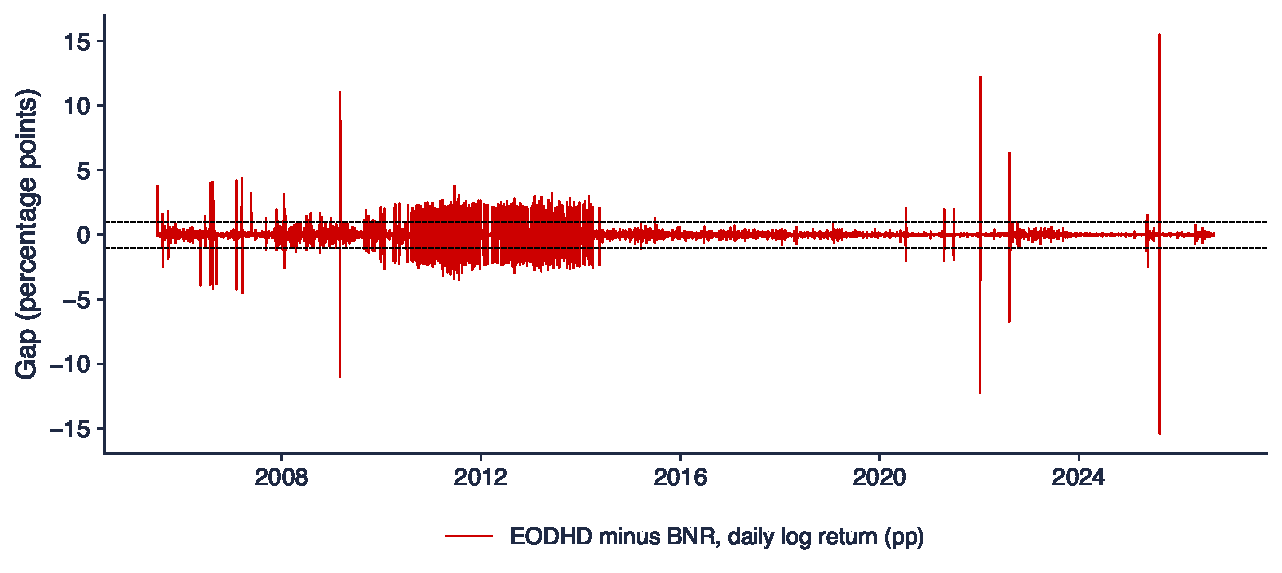
\includegraphics[width=0.96\textwidth,height=0.48\textheight,keepaspectratio]{ch1_sem_b1.pdf}
\end{center}
\vspace{-2mm}
\begin{itemize}
    \item 5\,154 de zile comune; în 412 dintre ele (8{,}0\%) diferența depășește un punct procentual; cele mai multe în 2011 (107 zile)
    \item Cele mai mari diferențe: 13 august 2025 (EODHD $15{,}4\%$, BNR $-0{,}10\%$), 14 august 2025 (EODHD $-15{,}4\%$, BNR $-0{,}01\%$)
    \item Volatilitatea: BNR 4{,}5\%, EODHD 13{,}4\%, EODHD fără zilele eronate 4{,}7\%
    \item Interpretare: cursul BNR, sursa primară a cifrei; seria EODHD ar multiplica de 3{,}0 ori riscul valutar măsurat
\end{itemize}\quantlet{SFM\_ch1\_seminar}{\qlurl{SFM_ch1_seminar}}
\end{frame}

\begin{frame}{B2: este pozitiv randamentul mediu al BET? [Rezolvat]}
\itemsize{\footnotesize}
\begin{itemize}
\item \textbf{Întrebarea}: este randamentul zilnic mediu al BET semnificativ diferit de zero în 2015--2026?
\item \textbf{Date}: închiderile BET, 2015--2026, randamente logaritmice zilnice în \%
\item \textbf{Cerințe}
\begin{enumerate}
    \item Calculați media, abaterea standard, asimetria, excesul de boltire, minimul (cu data lui) și maximul randamentelor logaritmice zilnice.
    \item Anualizați media și abaterea standard cu numărul real de observații pe an.
    \item Calculați eroarea standard a mediei anuale, intervalul de încredere 95\% și statistica $z$ pentru $H_0$: media $= 0$.
    \item Interpretare: seamănă histograma cu distribuția Normală?
    \item Interpretare: ce informație îi oferă intervalul de încredere unui investitor?
\end{enumerate}
\item \textbf{Raportați}: un tabel de statistici, intervalul de încredere, $z$ și $p$, două fraze de interpretare
\item Notebook: secțiunea B2
\end{itemize}
\end{frame}

\begin{frame}{B2: rezolvare [Rezolvat]}
\itemsize{\footnotesize}
\begin{columns}[T]
\begin{column}{0.50\textwidth}
\begin{center}
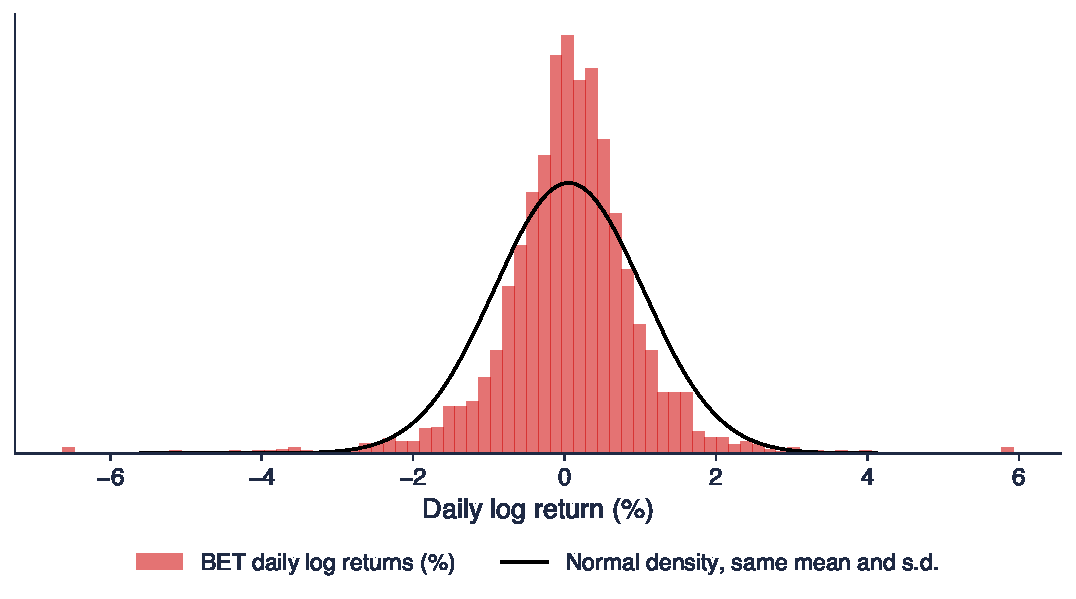
\includegraphics[width=1.0\textwidth,height=0.55\textheight,keepaspectratio]{ch1_sem_b2.pdf}
\end{center}
\vspace{-2mm}

\end{column}
\begin{column}{0.48\textwidth}
\begin{itemize}
    \item $n = 2\,925$ zile, 250 pe an; media $0{,}053\%$, abaterea std. $0{,}98\%$
    \item Asimetria $-1{,}41$, excesul de boltire $17{,}8$; cea mai slabă zi $-11{,}9\%$ pe 19 decembrie 2018, cea mai bună $6{,}8\%$
    \item Anual: media 13{,}2\%, volatilitatea 15{,}5\%; SE $= 15{,}5/\sqrt{11{,}7} = 4{,}5\%$
    \item Intervalul de încredere 95\%: [4{,}3\%; 22{,}1\%]; $z = 2{,}91$, $p = 0{,}004$: respingem ipoteza mediei zero la 5\%
    \item Interpretare: centru mai înalt și cozi mai groase decît distribuția Normală; media este pozitivă, dar se poate afla oriunde între 4{,}3\% și 22{,}1\% pe an
\end{itemize}
\end{column}
\end{columns}\quantlet{SFM\_ch1\_seminar}{\qlurl{SFM_ch1_seminar}}
\end{frame}

\begin{frame}{B3: încă patru piețe [Propus]}
\itemsize{\footnotesize}
\begin{itemize}
\item \textbf{Întrebarea}: care dintre S\&P 500, DAX, Bitcoin și Banca Transilvania au un randament mediu semnificativ peste zero?
\item \textbf{Date}: randamente logaritmice zilnice, 2015--2026, fiecare serie pe propriul calendar; model: B2
\item \textbf{Cerințe}
\begin{enumerate}
    \item Repetați pașii 1--3 din B2 pentru fiecare dintre cele patru serii.
    \item Reuniți într-un tabel media anuală, volatilitatea, intervalul de încredere și valoarea $p$ pentru toate cele cinci serii (inclusiv BET).
    \item Interpretare: de ce intervalul Bitcoin este mult mai larg decît cel al S\&P 500, deși ambele acoperă aceiași ani?
\end{enumerate}
\item \textbf{Raportați}: un tabel și două fraze
\item Notebook: secțiunea B3
\end{itemize}
\end{frame}

\ifsolutions
\begin{frame}{B3: rezolvare [Propus]}
\itemsize{\footnotesize}
\begin{center}
\footnotesize
\begin{tabular}{lrrrrr}
\toprule
Seria & Media \% & Vol. \% & SE \% & Interval 95\% & $p$ \\
\midrule
BET & $13{,}2$ & $15{,}5$ & $4{,}5$ & [$4{,}3$; $22{,}1$] & $0{,}004$ \\
S\&P 500 & $11{,}2$ & $17{,}7$ & $5{,}2$ & [$1{,}1$; $21{,}4$] & $0{,}030$ \\
DAX & $8{,}1$ & $19{,}1$ & $5{,}6$ & [$-2{,}8$; $19{,}1$] & $0{,}144$ \\
Bitcoin & $47{,}4$ & $66{,}7$ & $19{,}5$ & [$9{,}2$; $85{,}6$] & $0{,}015$ \\
Banca Transilvania & $24{,}2$ & $25{,}5$ & $7{,}5$ & [$9{,}6$; $38{,}8$] & $0{,}001$ \\
\bottomrule
\end{tabular}
\end{center}
\begin{itemize}
    \item Semnificative la 5\%: toate seriile al căror interval exclude zero; intervalul DAX conține zero
    \item Interpretare: SE $= \sigma_{\text{an}}/\sqrt{Y}$ cu același $Y$; volatilitatea Bitcoin este de 3{,}8 ori mai mare decît cea a S\&P 500, iar intervalul este de tot atîtea ori mai larg
\end{itemize}\quantlet{SFM\_ch1\_seminar}{\qlurl{SFM_ch1_seminar}}
\end{frame}
\fi

\begin{frame}{B4: cît de precis este raportul Sharpe? [Rezolvat]}
\itemsize{\footnotesize}
\begin{itemize}
\item \textbf{Întrebarea}: cît de precis se estimează raportul Sharpe al S\&P 500 din datele 2015--2026?
\item \textbf{Date}: închiderile S\&P 500, randamente simple zilnice, $r_f = 0$
\item \textbf{Cerințe}
\begin{enumerate}
    \item Calculați media zilnică, abaterea standard și raportul Sharpe zilnic, apoi anualizați raportul Sharpe.
    \item Calculați eroarea standard după \refLo{} și intervalul de încredere 95\%.
    \item Aplicați bootstrap raportului Sharpe, cu 2000 de reeșantionări ale zilelor, și calculați percentilele 2,5\% și 97,5\%.
    \item Interpretare: ar putea raportul Sharpe adevărat al S\&P 500 să fie sub 0,25?
\end{enumerate}
\item \textbf{Raportați}: raportul Sharpe, două intervale și o frază
\item Notebook: secțiunea B4
\end{itemize}
\end{frame}

\begin{frame}{B4: rezolvare [Rezolvat]}
\itemsize{\footnotesize}
\begin{columns}[T]
\begin{column}{0.50\textwidth}
\begin{center}
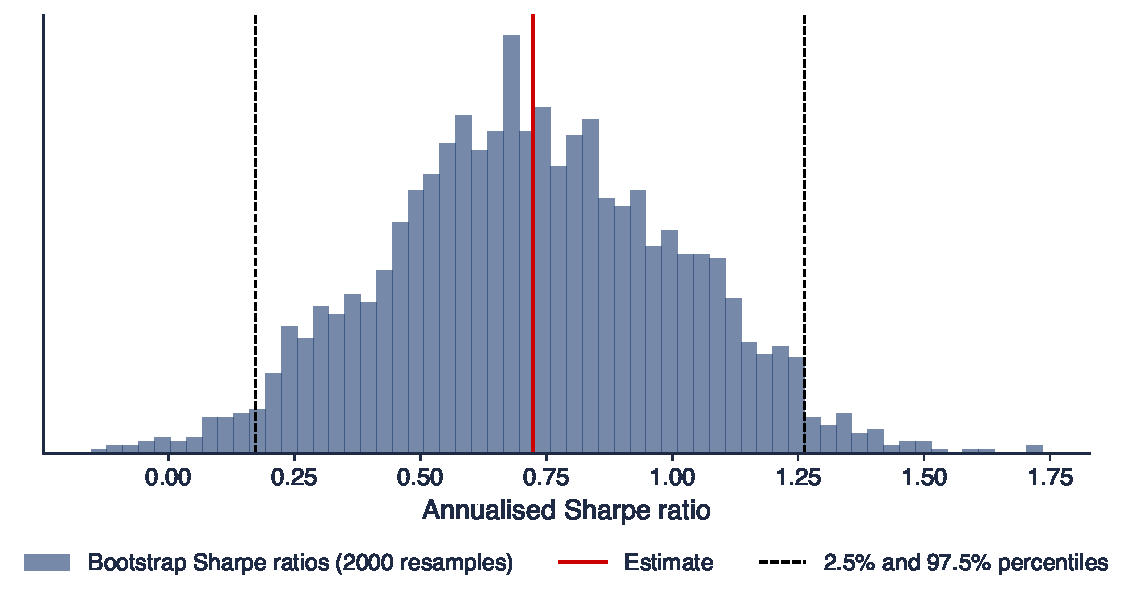
\includegraphics[width=1.0\textwidth,height=0.55\textheight,keepaspectratio]{ch1_sem_b4.pdf}
\end{center}
\vspace{-2mm}

\end{column}
\begin{column}{0.48\textwidth}
\begin{itemize}
    \item $n = 2\,943$, $q = 251{,}5$; media zilnică $0{,}0508\%$, abaterea std. $1{,}113\%$, SR zilnic $0{,}0457$
    \item SR anual $= 0{,}0457 \times 15{,}86 = 0{,}72$
    \item Lo: SE $= \sqrt{(1 + 0{,}0457^2/2)/2\,943} \times 15{,}86 = 0{,}29$; intervalul de încredere [$0{,}15$; $1{,}30$]
    \item Bootstrap: [$0{,}17$; $1{,}26$], foarte apropiat
    \item Interpretare: da; orice valoare de la $0{,}17$ la $1{,}26$ este compatibilă cu datele
\end{itemize}
\end{column}
\end{columns}\quantlet{SFM\_ch1\_seminar}{\qlurl{SFM_ch1_seminar}}
\end{frame}

\begin{frame}{B5: este Banca Transilvania mai bună decît BET? [Propus]}
\itemsize{\footnotesize}
\begin{itemize}
\item \textbf{Întrebarea}: este raportul Sharpe al TLV semnificativ mai mare decît cel al indicelui BET?
\item \textbf{Date}: închiderea BET și închiderea ajustată TLV, 2015--2026, aliniate întîi pe zilele comune; model: B4
\item \textbf{Cerințe}
\begin{enumerate}
    \item Aliniați cele două serii de prețuri pe zilele lor comune, apoi calculați randamentele simple zilnice.
    \item Calculați cele două rapoarte Sharpe anualizate, cu erorile standard Lo.
    \item Aplicați bootstrap diferenței dintre cele două rapoarte Sharpe, reeșantionînd aceleași zile pentru ambele serii.
    \item Interpretare: de ce trebuie reeșantionate zilele în perechi?
\end{enumerate}
\item \textbf{Raportați}: cele două rapoarte Sharpe, diferența cu intervalul ei, o frază
\item Notebook: secțiunea B5
\end{itemize}
\end{frame}

\ifsolutions
\begin{frame}{B5: rezolvare [Propus]}
\itemsize{\footnotesize}
\begin{itemize}
    \item 2\,674 de zile comune; SR BET $0{,}93$ (SE $0{,}29$), SR TLV $1{,}08$ (SE $0{,}29$)
    \item Diferența TLV $-$ BET $= 0{,}15$; intervalul bootstrap 95\% pe perechi, [$-0{,}24$; $0{,}53$], conține zero
    \item Nicio diferență semnificativă
    \item Interpretare: cele două serii de randamente sînt corelate ($\rho = 0{,}76$); reeșantionarea zilelor în perechi păstrează corelația, ceea ce face diferența mai precisă decît sugerează două intervale separate
\end{itemize}\quantlet{SFM\_ch1\_seminar}{\qlurl{SFM_ch1_seminar}}
\end{frame}
\fi

\begin{frame}{B6: cea mai adîncă cădere a BET [Rezolvat]}
\itemsize{\footnotesize}
\begin{itemize}
\item \textbf{Întrebarea}: care au fost adîncimea și durata celei mai mari căderi a BET de la lansare?
\item \textbf{Date}: închiderile oficiale BET din 19 septembrie 1997; pentru raportul Calmar, 2015--2026
\item \textbf{Cerințe}
\begin{enumerate}
    \item Calculați seria drawdown-urilor și drawdown-ul maxim, cu datele vîrfului, minimului și revenirii.
    \item Calculați cîștigul necesar pentru revenirea de la minim și ponderea zilelor petrecute cu peste 20\% sub vîrf.
    \item Calculați CAGR, MDD și raportul Calmar pentru 2015--2026.
    \item Interpretare: ce adaugă drawdown-ul la ceea ce ne spune deja volatilitatea?
\end{enumerate}
\item \textbf{Raportați}: MDD cu trei date, două procente, trei indicatori, o frază
\item Notebook: secțiunea B6
\end{itemize}
\end{frame}

\begin{frame}{B6: rezolvare [Rezolvat]}
\itemsize{\footnotesize}
\begin{center}
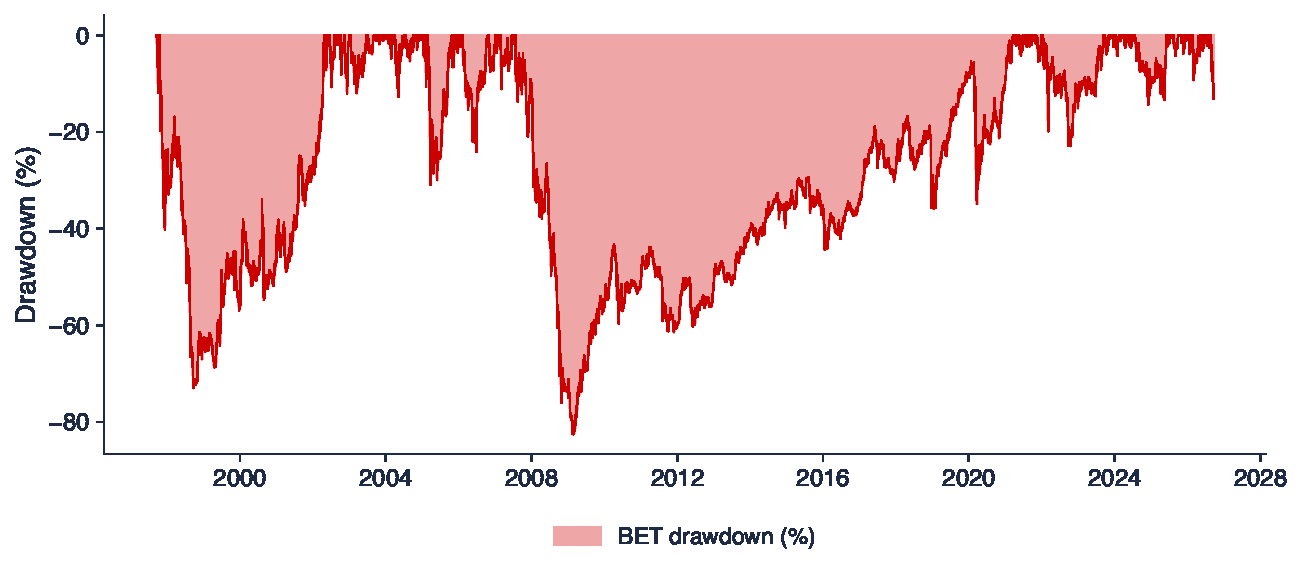
\includegraphics[width=0.96\textwidth,height=0.48\textheight,keepaspectratio]{ch1_sem_b6.pdf}
\end{center}
\vspace{-2mm}
\begin{itemize}
    \item MDD $-82{,}5\%$: de la 10\,814 puncte pe 24 iulie 2007 la 1\,887 pe 25 februarie 2009; vechiul vîrf a fost atins din nou pe 16 martie 2021, după 13{,}6 ani
    \item De la minim era nevoie de un cîștig de $473\%$; 56\% din toate zilele au fost cu peste 20\% sub vîrf
    \item 2015--2026: CAGR 14{,}1\%, MDD $-31{,}1\%$ (23 ianuarie 2020 -- 23 martie 2020), Calmar $= 14{,}1/31{,}1 = 0{,}45$
    \item Interpretare: volatilitatea ignoră ordinea randamentelor; drawdown-ul arată cît timp rămîne investitorul sub vîrful anterior (underwater)
\end{itemize}\quantlet{SFM\_ch1\_seminar}{\qlurl{SFM_ch1_seminar}}
\end{frame}

\begin{frame}{B7: Bitcoin, OMV Petrom și volatility drag [Propus]}
\itemsize{\footnotesize}
\begin{itemize}
\item \textbf{Întrebarea}: ce arată drawdown-urile și volatility drag pentru Bitcoin și SNP?
\item \textbf{Date}: închiderea Bitcoin și închiderea ajustată SNP, 2015--2026; model: B6
\item \textbf{Cerințe}
\begin{enumerate}
    \item Calculați MDD pentru fiecare serie, cu datele vîrfului, minimului și revenirii.
    \item Calculați CAGR și raportul Calmar pentru fiecare serie.
    \item Calculați media anuală aritmetică a randamentelor simple, media anuală a randamentelor logaritmice și diferența lor.
    \item Comparați diferența cu $\sigma^2/2$, folosind volatilitatea anuală a randamentelor simple.
    \item Interpretare: pentru care dintre cele două active este volatility drag important pentru un investitor pe termen lung?
\end{enumerate}
\item \textbf{Raportați}: un tabel cu MDD, date, CAGR, Calmar, cele două medii, volatility drag și $\sigma^2/2$, o frază
\item Notebook: secțiunea B7
\end{itemize}
\end{frame}

\ifsolutions
\begin{frame}{B7: rezolvare [Propus]}
\itemsize{\footnotesize}
\begin{center}
\footnotesize
\begin{tabular}{lrrrrrrr}
\toprule
Seria & MDD \% & CAGR \% & Calmar & Aritm. \% & Log \% & Drag \% & $\sigma^2/2$ \% \\
\midrule
Bitcoin & $-83{,}4$ & $60{,}6$ & $0{,}73$ & $69{,}5$ & $47{,}4$ & $22{,}13$ & $21{,}93$ \\
OMV Petrom & $-45{,}4$ & $19{,}7$ & $0{,}43$ & $20{,}8$ & $18{,}0$ & $2{,}73$ & $2{,}71$ \\
\bottomrule
\end{tabular}
\end{center}
\begin{itemize}
    \item Bitcoin: 16 decembrie 2017 -- 15 decembrie 2018, cu revenire pe 30 noiembrie 2020; SNP: 1 ianuarie 2015 -- 12 februarie 2016, cu revenire pe 20 septembrie 2018
    \item Volatility drag și $\sigma^2/2$ diferă cu cel mult 0{,}20 puncte procentuale
    \item Interpretare: pentru Bitcoin, volatility drag reprezintă 32\% din media aritmetică; pentru SNP este mic
\end{itemize}\quantlet{SFM\_ch1\_seminar}{\qlurl{SFM_ch1_seminar}}
\end{frame}
\fi


%=============================================================================
\section{Partea C: întrebări deschise și critica unui răspuns generat de AI}
%=============================================================================

\begin{frame}{C1: persistă rapoartele Sharpe? [Propus]}
\itemsize{\footnotesize}
\begin{itemize}
\item \textbf{Întrebarea}: are o acțiune BVB cu un raport Sharpe mare în 2015--2020 un raport Sharpe mare și în 2021--2026?
\item \textbf{Date}: închiderile ajustate TLV, SNP, BRD, TGN, SNG, SNN, 2015--2026; modele: B4, B6
\item \textbf{Cerințe}
\begin{enumerate}
    \item Calculați raportul Sharpe anualizat și eroarea lui standard pentru fiecare acțiune în fiecare jumătate.
    \item Calculați corelația rangurilor Spearman între rapoartele Sharpe din cele două jumătăți.
    \item Propuneți o modalitate de a face răspunsul mai robust (mai multe acțiuni, alți indicatori, alte ferestre).
    \item Interpretare: ce ne pot spune șase acțiuni despre persistență?
\end{enumerate}
\item \textbf{Raportați}: un tabel, corelația rangurilor cu valoarea $p$, un scurt plan de proiect
\item Notebook: secțiunea C1
\end{itemize}
\end{frame}

\ifsolutions
\begin{frame}{C1: analiză de referință [Propus]}
\itemsize{\footnotesize}
\begin{center}
\footnotesize
\begin{tabular}{lrrrr}
\toprule
Acțiunea & SR 2015--2020 & SE & SR 2021--2026 & SE \\
\midrule
Banca Transilvania & $0{,}91$ & $0{,}41$ & $1{,}34$ & $0{,}42$ \\
OMV Petrom & $0{,}26$ & $0{,}41$ & $1{,}75$ & $0{,}42$ \\
BRD & $0{,}71$ & $0{,}41$ & $0{,}96$ & $0{,}42$ \\
Transgaz & $0{,}63$ & $0{,}41$ & $1{,}27$ & $0{,}42$ \\
Romgaz & $0{,}52$ & $0{,}41$ & $1{,}63$ & $0{,}42$ \\
Nuclearelectrica & $1{,}31$ & $0{,}41$ & $1{,}23$ & $0{,}42$ \\
\bottomrule
\end{tabular}
\end{center}
\begin{itemize}
    \item Corelația rangurilor Spearman $-0{,}71$ ($p = 0{,}11$, $n = 6$): nicio dovadă de persistență; mai degrabă o inversare
    \item Fiecare raport Sharpe estimat pe o jumătate de eșantion are o eroare standard de circa $0{,}41$: clasamentele sînt în mare parte zgomot
    \item Direcții de proiect: toate acțiunile lichide BVB, ferestre mobile de trei ani, Sortino și Calmar, comparație cu \refHLZ
\end{itemize}\quantlet{SFM\_ch1\_seminar}{\qlurl{SFM_ch1_seminar}}
\end{frame}
\fi

\begin{frame}{C2: verificarea unui răspuns generat de AI [Propus]}
\itemsize{\scriptsize}
\begin{itemize}
    \item Un student a întrebat un asistent AI: „Compară riscul și performanța Bitcoin și ale BET în 2015--2026.” Răspunsul:
    \item \aiprompt{(a) Volatilitatea zilnică a Bitcoin este 3{,}49\%, deci volatilitatea anuală este 3{,}49\% x sqrt(252) = 55{,}4\%.}
    \item \aiprompt{(b) Raportul Sharpe al Bitcoin (1{,}05) este mai mare decît al BET (0{,}93), ceea ce dovedește că Bitcoin este investiția mai bună.}
    \item \aiprompt{(c) Drawdown-ul maxim al Bitcoin este cel mai slab randament zilnic, -46{,}5\%.}
    \item \aiprompt{(d) Pentru un portofoliu 50/50, randamentul logaritmic este exact media celor două randamente logaritmice.}
    \item \aiprompt{(e) Pentru acțiunile BVB, ca TLV, am folosit coloana close, care este prețul oficial.}
    \item Cerințe
    \begin{itemize}
        \item 1. Pentru fiecare afirmație, precizați dacă este corectă; dacă nu este, formulați afirmația corectă și, unde este posibil, dați cifra corectă din notebook (secțiunea C2).
        \item 2. Raportați: o listă de cinci verdicte, fiecare cu un rînd de justificare.
    \end{itemize}
\end{itemize}
\end{frame}

\ifsolutions
\begin{frame}{C2: rezolvare [Propus]}
\itemsize{\footnotesize}
\begin{itemize}
    \item (a) Factor greșit: Bitcoin se tranzacționează aproximativ 365 de zile pe an; $3{,}49\% \times \sqrt{365} = 66{,}7\%$, nu 55{,}4\%
    \item (b) Nu este dovedit: SE $\approx 0{,}29$ pentru fiecare raport Sharpe, deci diferența dintre cele două estimări se încadrează în zgomot; iar rapoartele Sharpe din trecut nu le garantează pe cele viitoare
    \item (c) Definiție greșită: MDD este cea mai mare cădere de la vîrf la minim, $-83{,}4\%$; cea mai slabă zi a fost $-46{,}5\%$ (randament logaritmic)
    \item (d) Greșit: $R_p = \sum_i w_i R_i$ este exact; $r_p = \ln(\sum_i w_i e^{r_i})$ diferă de $\sum_i w_i r_i$
    \item (e) Coloană greșită: prețul de închidere TLV crește brusc cu $+230\%$ (logaritmic) pe 16 august 2022, din cauza unei consolidări a acțiunilor; volatilitatea calculată din close este 73{,}1\%, față de 25{,}5\% din prețul ajustat
\end{itemize}\quantlet{SFM\_ch1\_seminar}{\qlurl{SFM_ch1_seminar}}
\end{frame}
\fi


%=============================================================================
\section{Încheiere}
%=============================================================================

\begin{frame}{Idei de reținut}
\itemsize{\small}
\begin{itemize}
    \item Verificați datele înainte de calcule: sursa, prețurile ajustate, o a doua serie
    \item Randamentele logaritmice se adună în timp; cele simple se adună între active
    \item Randamentele medii și rapoartele Sharpe au intervale de încredere largi: raportați-le
    \item Drawdown-ul și volatility drag arată ceea ce volatilitatea singură nu arată
    \item Un răspuns generat de AI este o ciornă: verificați fiecare factor, definiție și coloană
\end{itemize}
\end{frame}

\begin{frame}{După seminar}
\itemsize{\small}
\begin{itemize}
    \item Cursul 1 dezvoltă fiecare temă de azi: calitatea datelor, randamente, anualizare, statistici descriptive și indicatori de performanță
    \item Încercați cerințele [Propus] în notebook; rezolvările se discută la seminar
    \item C1 poate deveni un proiect de echipă: mai multe acțiuni, ferestre mobile, alți indicatori
    \item Lectură: \refFHH, cap.~11; exerciții rezolvate: \refFHHex
\end{itemize}
\end{frame}


%=============================================================================
\section{Bibliografie}
%=============================================================================

\begin{frame}{Bibliografie}
\itemsize{\tiny}
\begin{itemize}
    \item Borak, S., Härdle, W.K., López-Cabrera, B. (2013). \href{https://doi.org/10.1007/978-3-642-33929-5}{\textit{Statistics of Financial Markets: Exercises and Solutions}}, 2nd ed. Springer.
    \item Franke, J., Härdle, W.K., Hafner, C.M. (2019). \href{https://doi.org/10.1007/978-3-030-13751-9}{\textit{Statistics of Financial Markets: An Introduction}}, 5th ed. Springer.
    \item Harvey, C.R., Liu, Y., Zhu, H. (2016). \href{https://doi.org/10.1093/rfs/hhv059}{\ldots and the cross-section of expected returns}. \textit{Review of Financial Studies}, 29(1), 5--68.
    \item Lo, A.W. (2002). \href{https://doi.org/10.2469/faj.v58.n4.2453}{The statistics of Sharpe ratios}. \textit{Financial Analysts Journal}, 58(4), 36--52.
    \item Sharpe, W.F. (1994). \href{https://doi.org/10.3905/jpm.1994.409501}{The Sharpe ratio}. \textit{Journal of Portfolio Management}, 21(1), 49--58.
    \item Sortino, F.A., van der Meer, R. (1991). \href{https://doi.org/10.3905/jpm.1991.409343}{Downside risk}. \textit{Journal of Portfolio Management}, 17(4), 27--31.
\end{itemize}
\end{frame}

\end{document}
